%% ----------------------------------------------------------------
%% Thesis.tex -- MAIN FILE (the one that you compile with LaTeX)
%% ---------------------------------------------------------------- 

% Set up the document
\documentclass[a4paper, 12pt, oneside]{uet_thesis}  % Use the "Thesis" style, based on the ECS Thesis style by Steve Gunn
\graphicspath{{Figures/}}  % Location of the graphics files (set up for graphics to be in PDF format)
\oddsidemargin=1.2in

% Include any extra LaTeX packages required
\usepackage[square, numbers, comma, sort&compress]{natbib}  % Use the "Natbib" style for the references in the Bibliography

\usepackage{verbatim}  % Needed for the "comment" environment to make LaTeX comments

\usepackage{vector}  % Allows "\bvec{}" and "\buvec{}" for "blackboard" style bold vectors in maths

\usepackage{url}
\usepackage{float}
\usepackage{natbib}


\hypersetup{urlcolor=blue, colorlinks=true}  % Colours hyperlinks in blue, but this can be distracting if there are many links.

% remove the unnecessary spacing before and after the headings/subheadings
\usepackage[compact]{titlesec}
\titlespacing{\section}{0pt}{*0}{*0}
\titlespacing{\subsection}{0pt}{*0}{*0}
\titlespacing{\subsubsection}{0pt}{*0}{*0}

\setlength{\parskip}{6pt}
%\setlength{\parsep}{0pt}
%\setlength{\headsep}{0pt}
%\setlength{\topskip}{0pt}

\usepackage{listings}
\usepackage{color} %red, green, blue, yellow, cyan, magenta, black, white
\definecolor{mygreen}{RGB}{28,172,0} % color values Red, Green, Blue
\definecolor{mylilas}{RGB}{170,55,241}

\usepackage{amsmath} % for "align*" environment
\usepackage[table,xcdraw]{xcolor}

%% ----------------------------------------------------------------
\begin{document}
\frontmatter	  % Begin Roman style (i, ii, iii, iv...) page numbering

% Set up the Title Page
\title  {Development of test bench model for evaluating the efficiency of induction motors}
\session {2017 -- Fall}
\advisor {Dr. Muhammad Tahir Izhar}
\authors {
Arslan Ahmad ~~~ 2017(F)-MS-EE-32 }

\addresses  {\deptname \\ \univname}  % Do not change this here, instead these must be set in the "Thesis.cls" file, please look through it instead
\date       {\today}
\subject    {}
\keywords   {}

\maketitle
%% ----------------------------------------------------------------

\setstretch{1.3}  % It is better to have smaller font and larger line spacing than the other way round

% Define the page headers using the FancyHdr package and set up for one-sided printing
\fancyhead{}  % Clears all page headers and footers
\rhead{\thepage}  % Sets the right side header to show the page number
\lhead{}  % Clears the left side page header

\pagestyle{fancy}  % Finally, use the "fancy" page style to implement the FancyHdr headers


%% Select only one of the certification pages  
\CertificationMSc{}
%\CertificationBSc{}
\clearpage  % Certification ended, now start a new page


%% ----------------------------------------------------------------
% Declaration Page required for the Thesis, your institution may give you a different text to place here
\Declaration{
%\addtocontents{toc}{\vspace{1em}}  % Add a gap in the Contents, for aesthetics

I declare that the work contained in this thesis is my own, except where explicitly stated otherwise. In addition this work has not been submitted to obtain another degree or professional qualification.

\bigskip

Signed:~~ \rule[0em]{10em}{1.0pt} \\ % This prints a line for the signature 
Date:~~~~ \rule[0em]{10em}{1.0pt}  % This prints a line to write the date
}
\clearpage     % Declaration ended, now start a new page

%% ----------------------------------------------------------------

\setstretch{1.3}  % Reset the line-spacing to 1.3 for body text (if it has changed)

% The Acknowledgements page, for thanking everyone
\acknowledgements{
%\addtocontents{toc}{\vspace{1em}}  % Add a gap in the Contents, for aesthetics

I would express a deep sense of gratitude and respect to my Advisor, Dr. Muhammad Tahir Izhar for his guidance, motivation and help, and consider myself extremely lucky to work under his guidance. I would also like to thank all the faculty members of my department and KICS department for their pieces of advise and help that they provided me.

}
\clearpage  % End of the Acknowledgements

%% ----------------------------------------------------------------
% End of the pre-able, contents and lists of things
% Begin the Dedication page
\setstretch{1.3}  % Return the line spacing back to 1.3
\pagestyle{empty}  % Page style needs to be empty for this page
\dedicatory{Dedicated To My Parents, \\Who Always Sacrifice Their Dreams for My Betterment}


%% ----------------------------------------------------------------
\pagestyle{fancy}  %The page style headers have been "empty" all this time, now use the "fancy" headers as defined before to bring them back

%% ----------------------------------------------------------------
\lhead{\emph{Contents}}  % Set the left side page header to "Contents"
\tableofcontents  % Write out the Table of Contents

%% ----------------------------------------------------------------
\lhead{\emph{List of Figures}}  % Set the left side page header to "List if Figures"
\listoffigures  % Write out the List of Figures

%% ----------------------------------------------------------------
%\lhead{\emph{List of Tables}}  % Set the left side page header to "List of Tables"
%\listoftables  % Write out the List of Tables

%% ----------------------------------------------------------------
\setstretch{1.5}  % Set the line spacing to 1.5, this makes the following tables easier to read
%\clearpage  % Start a new page
%\lhead{\emph{Abbreviations}}  % Set the left side page header to "Abbreviations"
%\listofsymbols{ll}  % Include a list of Abbreviations (a table of two columns)
{
% \textbf{Acronym} & \textbf{W}hat (it) \textbf{S}tands \textbf{F}or \\
%\textbf{LAH} & \textbf{L}ist \textbf{A}bbreviations \textbf{H}ere \\
}

%% ----------------------------------------------------------------
% The Abstract Page
\addtotoc{Abstract}  % Add the "Abstract" page entry to the Contents
\abstract{
%\addtocontents{toc}{\vspace{1em}}  % Add a gap in the Contents, for aesthetics

Abstract.

}
\clearpage  % Abstract ended, start a new page


%% ----------------------------------------------------------------
\mainmatter	  % Begin normal, numeric (1,2,3...) page numbering
\pagestyle{fancy}  % Return the page headers back to the "fancy" style
\onehalfspacing
% Include the chapters of the thesis, as separate files
% Just uncomment the lines as you write the chapters

% Chapter 1
\setstretch{1.8}
\chapter{Introduction} % Write in your own chapter title
\label{Chapter1}
\lhead{Chapter 1. \emph{Introduction}} % Write in your own chapter title to set the page header

\section{Background}

Electric motors are an important invention of the modern era and comprise a major portion of the electric load of any country. Induction motors are the most commonly used type of motors, being used widely in industry, agriculture, domestic, municipal and commercial applications. In a domestic environment, they are found in many appliances, including but not limited to air conditioners, refrigerators, water pumps, and kitchen appliances (grinder, blender, etc.). In agriculture they are used as pumps, for watering the crops. In industry, they are found at different places according to the nature of industry, e.g. in textiles, they are using in weaving mills, in oil and gas, they are used in pumps, in assembly line, they are used to drive the belts, etc. According to the WEC (World Energy Council), in industrialized countries three main sectors are responsible for three quarters of electricity consumption: electric motors, 45 \%, lighting, about 15 \%, and home appliances and consumer electronics, also around 15 \%.Global energy consumption of electric motors is around 9000 TWh per year\cite{tandel2019energy}. These data show the impact that electric motors produce on electrical energy consumption. Therefore, the manufacturers in this sector are investing heavily in the energy efficiency of their products. The following figures show the statistical usage of electric machines [INSERT PIE CHARTS AND GRAPHS HERE].

\section{Switching to an efficient world}
From the above scenario, it is clear that induction machines comprise a major part of the total electric load of any country. So, the efficiency of these motors is an important parameter in controlling the total load. If the machines are replaced by more efficient ones, a large amount of energy can be saved.
\begin{figure}[htbp]
  \centering
    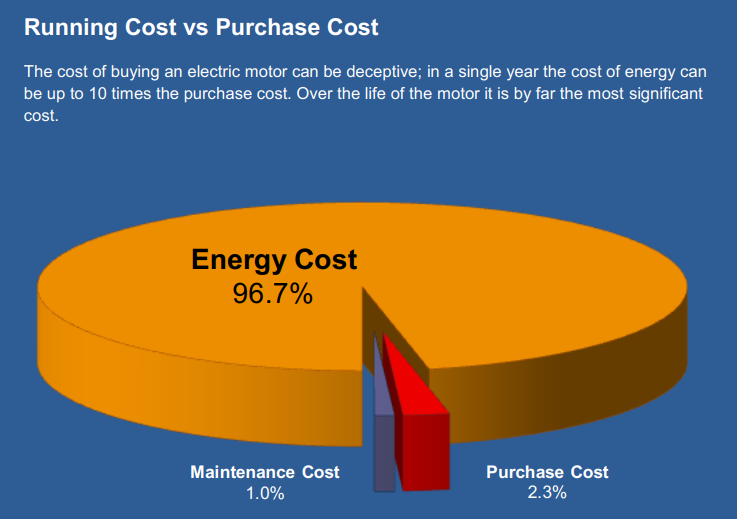
\includegraphics[width = 5in]{./Figures/MS/fig11.png}
    \rule{35em}{1.2pt}
  \caption{Running cost vs purchase cost of induction motors}
  \label{fig:Running cost vs purchase cost of induction motors}
\end{figure}
\begin{figure}[htbp]
  \centering
    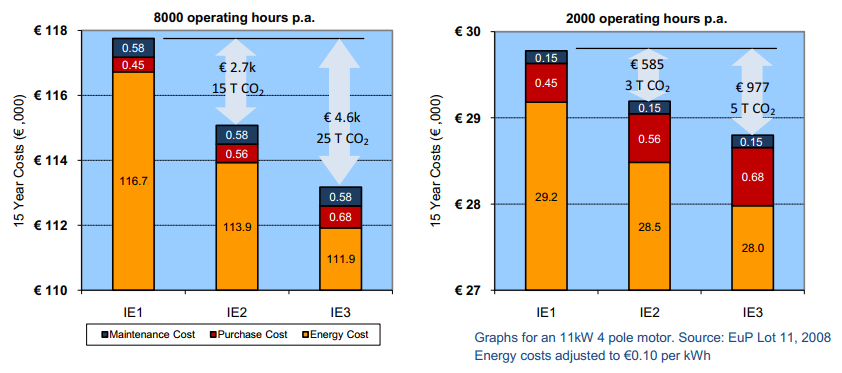
\includegraphics[width = 5in]{./Figures/MS/fig12.png}
    \rule{35em}{1.2pt}
  \caption{Cost comparison of IE1, IE2 and IE3 motors}
  \label{fig:Cost comparison of IE1, IE2 and IE3 motors}
\end{figure}
At 8000 operating hours per year, the additional cost of an IE2 motor is paid back in 7 months, with an IE3 motor paying back in 10 months. Even at only 2000 operating hours per year, the energy saving repays the capital in about 3 years\cite{caetano2018energy}.

\section{Domestic Use of Motors in Pakistan}
Motors are found in Pakistan in almost all the homes for water supply. This thesis particularly focuses on these motors. There are two main types of motor pumps available in the market:
\begin{itemize}
	\item Reciprocating pumps
	\item Centrifugal pumps
\end{itemize}
Reciprocating pumps are being used more while centrifugal pumps have recently entered the domestic market. They were previously commonly used in large setups like tube wells and municipal pumps.
\begin{figure}[htbp]
  \centering
    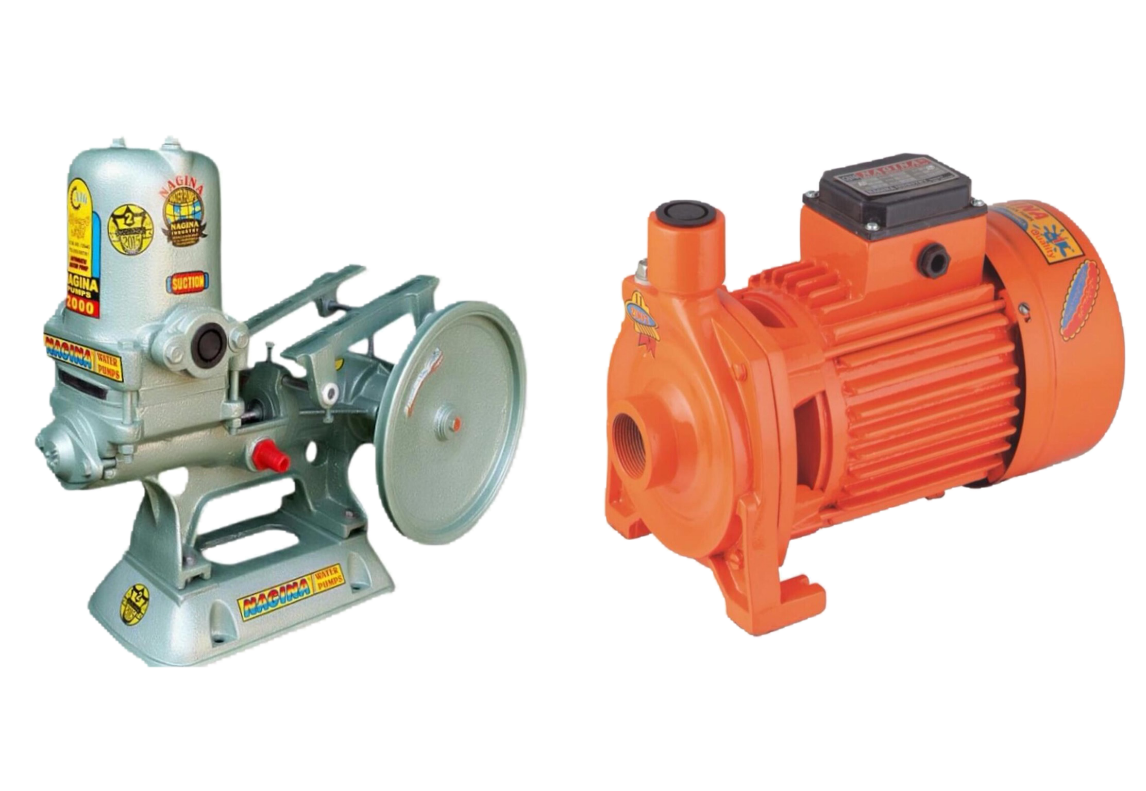
\includegraphics[width = 5in]{./Figures/MS/fig13.png}
    \rule{35em}{1.2pt}
  \caption{Reciprocating pump(left) vs Centrifugal pump(right)}
  \label{fig:Reciprocating pump(left) vs Centrifugal pump(right)}
\end{figure}
The local market in Pakistan for domestic motor pumps has not been following any international standards. IEC endorsed its efficiency standards to Pakistan in 2017, which has opened new opportunities for the manufacturers to use improved testing methods and identify the possible causes of losses and efficiency and improve them. This thesis also focuses on utilizing the IEC standards to create a standardized test bench which can be made available in the local market for low costs. Currently, such setups cost around 25,000 USD for setups with capacity to test 10 hp motors. 

\section{Objectives}
The main goal of the project was to develop a test bench for evaluating the efficiency of small induction motors simular to those used in domesting water pumping applications. This work of this project will be extended to design test benches that will be used to evaluate the efficiences of the motors available in the Pakistan local market, under the HEC TDF-02-173 project, which aims at development of a testbench for motor/pump strings so they can be tested and certified according to international standards. This project is also a part of the HEC project.
\begin{figure}[htbp]
  \centering
    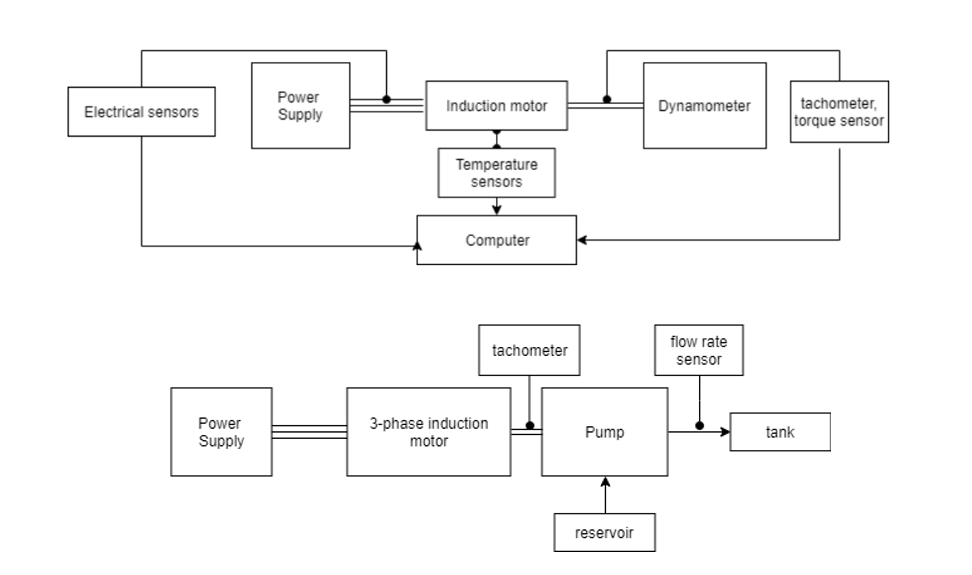
\includegraphics[width = 5in]{./Figures/MS/fig16.png}
    \rule{35em}{1.2pt}
  \caption{Scope of the HEC TDF-02-173 project.}
  \label{fig:Scope of the HEC TDF-02-173 project.}
\end{figure}
\begin{figure}[htbp]
  \centering
    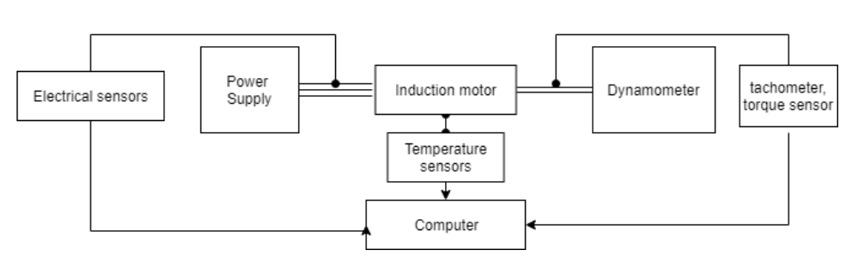
\includegraphics[width = 5in]{./Figures/MS/fig17.png}
    \rule{35em}{1.2pt}
  \caption{Scope of this thesis project.}
  \label{fig:Scope of this thesis project.}
\end{figure}

\section{MEPS (Minimum Energy Performance Standards)}
MEPS is a set of policies in a country that defines minimum efficiencies for different appliances and machinery sold in that country. This trend was started by the USA with the energy policy act of 1992, in which a large number of machines were required to be upgraded to comply with the efficiency standards. This policy was implemented in 8 years, in different phases. Europe followed and the CEMEP (European Committee of Manufacturers of Electrical Machines and Power Electronics) also created a similar policy. Currently, the minimum efficiency requirements in the USA are IE3, while EU allows IE3 or IE2 motors with a VFD as it has increased efficiency. These efficiency classes are defined by the IEC 60034-30-1 standard. Some other countries that have also defined MEPS for a set of appliances e.g. Air Conditioners, Refrigerators, lighting equipment, etc. include, but not limited to, Australia, Brazil, Japan, China, New Zealand.   
In Pakistan, the National Energy Efficiency \& Conservation Authority (NEECA) is responsible for maintaining energy standards. Currently, it has defined rules for air conditioners, refrigerators, fluorescent bulbs and induction motors. For induction motors, since the standards have recently been applied, so the efficiency requirements are set a bit lower than international standards so allow the local manufacturers to catch up. e.g. the required minimum efficiency for an IE1 4-pole 50 Hz motor is 66 \%, while NEECA has set it to 62.7 \% for its phase-1.
\begin{figure}[htbp]
  \centering
    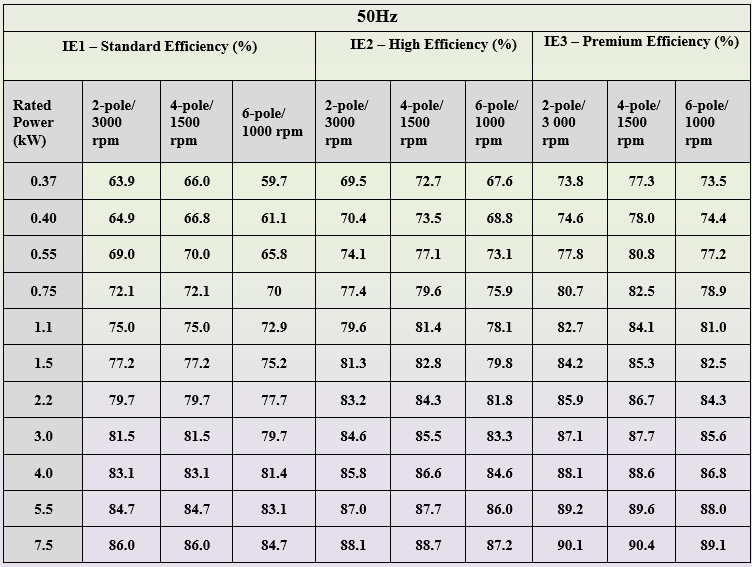
\includegraphics[width = 5in]{./Figures/MS/fig14.png}
    \rule{35em}{1.2pt}
  \caption{Minimum efficiencies for induction motors by IEC-60034-30}
  \label{fig:Minimum efficiencies for induction motors by IEC-60034-30}
\end{figure}
\begin{figure}[htbp]
  \centering
    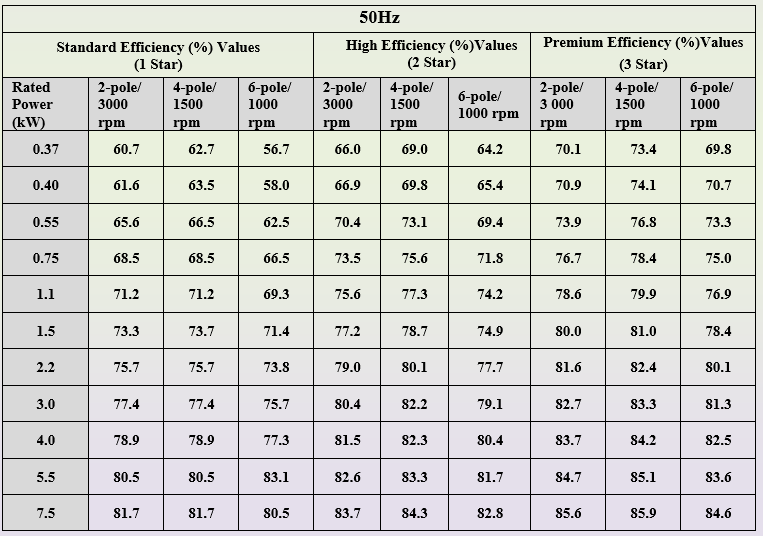
\includegraphics[width = 5in]{./Figures/MS/fig15.png}
    \rule{35em}{1.2pt}
  \caption{Modified minimum efficiencies for induction motors by NEECA}
  \label{fig:Modified minimum efficiencies for induction motors by NEECA}
\end{figure}

\section{Thesis Outline}
Chapter 2 of the thesis provides a brief overview of the literature behind the losses in the machines. Losses are categorized according to the IEC standard and another section that introduces the factors in machines that mainly cause these losses.
Chapter 3 gives and introduction to machine testing and also discusses the techniques used in this project. It also provides a provides the market estimated prices and quotations for the different types of sensors required for making a hardware setup
Chapter 4 is related to the algorithms, codes and flowcharts for the strategies used. The project was completely simulated in MATLAB and Simulink, where physical systems were designed in Simulink and algorithms were implemented using MATLAB scripts
Chapter 5 provides the results of the different tests performed and concluding remarks.
 % Introduction 
% Chapter 1
\setstretch{1.8}

\chapter{Literature Study of Induction Motors} % Write in your own chapter title
\label{Literature Study of Induction Motors}
\lhead{Chapter 2. \emph{Literature Study of Induction Motors}} % Write in your own chapter title to set the page header

\section{Induction motors}
In Present times, induction motors are the workhorse of the modern industry. They the most used type of electric machine in the industry as well as domestic use, since they are relatively low-cost and robust. Additionally, they are even appropriate for inflammable work environments such as sawmills and chemical factories\cite{esenozdemir2016}. Particularly, the advancement of the converter technology has enabled quite accurate control of the induction motors. Therefore, making it possible to use induction motors even in applications which involve accurate speed control. This section describes the working principles, structures and steady state equivalent circuit of an induction motor.

\section{Induction motor structure}
There are two main types of induction motors: 
\begin{itemize}
	\item Wound rotor induction motor 
	\item Squirrel Cage induction motor. 
\end{itemize}

This chapter focuses only on the latter one, because the test bench was implemented with a Squirrel Cage type induction motor. The assembly of a Squirrel cage induction motor consists of two major parts which are:
\begin{itemize}
	\item Stator winding 
	\item Rotor cage
\end{itemize}

These parts are shown in Figure 1 where portion of the induction motor body and stator has been cut. This exposes the laminated cage rotor mounted to the shaft and stator winding near it. Moreover, supplementary structures are added to the design of motor from time to time so as to gain some desired features depending on the application
\begin{figure}[htbp]
	\centering
		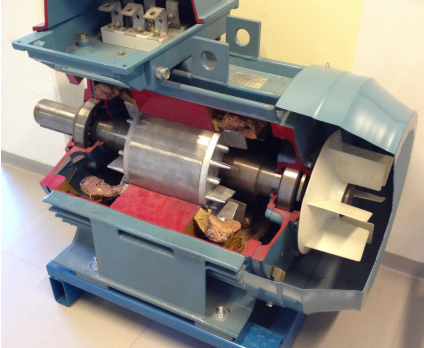
\includegraphics[width = 4.5in]{./Figures/MS/26.png}
		\rule{35em}{0.5pt}
	\caption{Cut-out of a squirrel cage induction motor}
	\label{fig:Cut-out of a squirrel cage induction motor}
\end{figure}

The cage rotor consists of bars constructed from a conductive substance. Typically, they are created from aluminum or copper and both sides of the bars are short circuited with shorting rings. The right side in Figure 2 illustrates the main construction of the cage used in the rotor.
\begin{figure}[htbp]
	\centering
		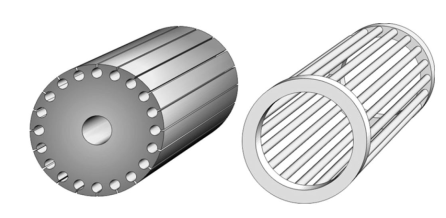
\includegraphics[width = 4.5in]{./Figures/MS/27.png}
		\rule{35em}{0.5pt}
	\caption{Laminated core(left) and steel structure(right)}
	\label{fig:Laminated core(left) and steel structure(right)}
\end{figure}

This sort of cage is next positioned inside a laminated core to reduce magnetic leakage and eddy current losses. Outer assembly of this laminated rotor core is shown on the left in Figure 2. Additionally, the conduction bars are typically not positioned entirely parallel to the orientation of the shaft, as shown in Figure 2, but slightly tilted. This practice is called skewing and it reduces cogging effect that might cause a blocked rotor situation. Additionally, this method minimizes the magnetic hum and sound produced by the motor. The illustrated rotor assembly is the most used in the field. However, altered variants as regards to the shape and size of the bars are used. Occasionally, even a double-cage rotor is used to achieve desired features. 

The other key element is the stator winding. Induction motor stator comprises wound coils. These are mostly made of ring-shaped copper wires or moulded flat copper structures. The coils are positioned in a laminated assembly as the cage rotor to avoid eddy current losses and to minimize magnetic leakage. Together, the rotor and the stator formulate a magnetic circuit. A rotating magnetic field is formed in the air gap between the stator and the rotor when a sinusoidal voltage is applied. The rotational speed of the magnetic field is called synchronous speed and defined as:
\begin{equation}
	n_s=(120*f_s)/p
\end{equation}
\begin{align*}
	\text{where:}\quad
	 f    &=  \text{frequency of applied voltage.} \\
	 p    &=  \text{number of poles.} \\
\end{align*}
A voltage is induced in the rotor bars according to the Faraday's law of induction due to this rotating magnetic field. Current begins to flow through the bars as they are shorted with shorting rings at both ends. Thus, creating a magnetic field in the rotor bars. However, a difference in the two magnetic fields is produced as the rotor sinusoidal current lags the stator current. This induces torque to the rotor bars causing rotational motion of the shaft.
The produced torque is proportional to the relative speed of the stator and rotor magnetic fields. In the absence of a difference, a stationary magnetic field is experienced by the rotor bars, and so, by Faraday’s law, no voltage will be induced, and hence, no torque is produced. So induction motors can never run at the synchronous speeds. This difference between synchronous speed and rotor speed si called slip and is defined as:
\begin{equation}
	s=(n_s-n_r)/n_s
\end{equation}
\begin{align*}
	\text{where:}\quad
	 n_s    &=  \text{synchronous speed.} \\
	 n_r    &=  \text{speed of rotor.} \\
\end{align*}

\section{Types of Losses}
According to the IEC standards\cite{iec6003421}, following are the types of losses in induction motors:
\begin{itemize}
\item Constant Losses
\subitem Iron(core) Losses
\subitem Friction Losses
\subitem Windage losses
\item Variable losses
\subitem Stator Copper(winding) losses
\subitem Rotor Copper(winding) losses
\subitem Stray or Additional load losses 
\end{itemize}

\begin{figure}[htbp]
	\centering
		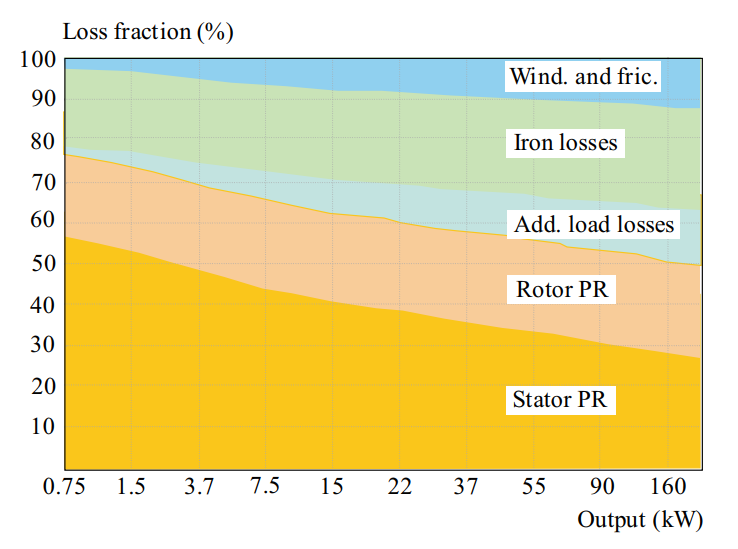
\includegraphics[width = 4.5in]{./Figures/MS/21.png}
		\rule{35em}{0.5pt}
	\caption{Typical loss distribution in induction motors}
	\label{fig:Typical loss distribution in induction motors}
\end{figure}

\subsection{Iron losses}
These are the losses in the active iron and additional no-load losses in other parts. They are divided into two losses:
-	Eddy current losses
-	Hysteresis losses
The eddy current losses are produced due to current flowing in the magnetic core, while hysteresis losses occur due to magnetization and demagnetization of the electromagnet.

Eddy current loss can be given by:
\begin{equation}
P_e=K_e * (B_max)^2 * f^2 * t^2 * V
\end{equation}
\begin{align*}
\text{where:}\quad
 K_e    &=  \text{eddy current constant.} \\
 B_{max}    &=  \text{flux density (Wb/m\textsuperscript{2}).} \\
 f    &=  \text{frequency .} \\
 t    &=  \text{material thickness.} \\
 V    &=  \text{volume.} \\
\end{align*}
So, eddy current loss mainly depends on the frequency and dimensions.

Hysteresis loss is given as:
\begin{equation}
P_b= \eta * (B_max)^n * V
\end{equation}
\begin{align*}
\text{where:}\quad
 \eta    &=  \text{Steinmetz hysteresis coefficient, depending on material .} \\
 B_{max}    &=  \text{flux density (Wb/m\textsuperscript{2}).} \\
 t    &=  \text{Steinmetz exponent, ranges from 1.5 to 2.5, depending on material.} \\
 f    &=  \text{frequency .} \\
 V    &=  \text{volume.} \\
\end{align*}
So hysteresis loss also depends on the frequency and dimensions.

\subsection{Friction Losses}
These are the losses due to friction in bearings, brushes, etc. and don't include any losses from separate lubricating systems.

\subsection{Windage Losses}
Theses are the losses due to aerodynamic friction in all parts of machine, including shaft mounted fans, etc.

\subsection{Winding or Copper Losses}
The I\textsuperscript{2}.R losses are known as copper losses or winding losses. These occur in the rotor and the stator. Their measurement is simple in case of stator, while for rotor, these are calculated using separation of losses method as it is not directly measurable.

\subsection{Additional Load Losses}
These are miscellaneous losses due to stray flux when machine is loaded, eddy current losses in winding conductors caused by load current dependent flux pulsations and additional brush losses caused by commutation, etc.

\section{Factors contributing towards motor efficiency}
Following are the factors mainly contributing towards a motor's efficiency\cite{manoharan2009review}:

\subsection{Active Material}
The active material is the main material in the motor that is responsible for electromechanical conversion. It is mostly copper or aluminium. The motor efficiency can be increased by increasing the active material, but this needs to be optimized for cost and weight.

\subsection{Lamination materials}
Instead of using a large block of iron as core, laminated thin sheets of iron are used to drastically reduce the eddy losses. High performacnce lamination materials(permeability, losses, and insulation)  can be used  to improve the efficiency further 

\subsection{Temperature levels of motor}
The stator and rotor I\textsuperscript{2}.R losses are directly proportional to the motor temperature levels. By designing the motor for better heat flow and heat transfer from active to non-active parts, the temperatures can be lowered, hence improving the efficiency.

\subsection{Stator and rotor geometries}
With careful optimization of stator and rotor geometries, the motor efficiency can be greatly enhanced. A non symmetric design will be prone to vibrations due to unbalancing, etc.

\subsection{Air gap dimensions}
Air gap dimensions are likewise an important item to be optimized to achieve improved efficiency without essentially increasing the overall material cost.

\subsection{Manufacturing Processes}
Optimization of manufacturing procedures is the one of the important factors to reduce stray-load losses, which are hard to foresee and, in general, merely to be determined by 
prototype testing

\subsection{Fan efficiency}
An efficient fan can help reduce friction and windage losses.

\subsection{Bearing efficiency}
By reducing the bearing friction, we can gain a small amount of improvement in efficiency.

\begin{figure}[htbp]
	\centering
		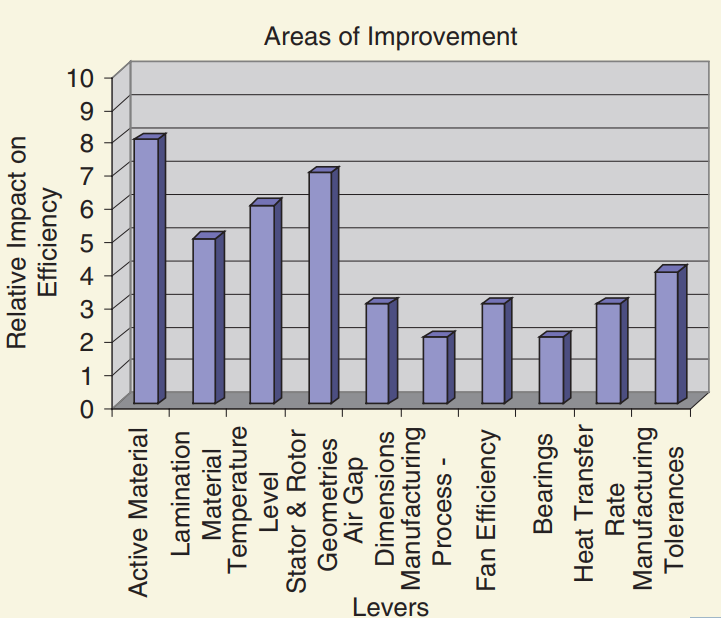
\includegraphics[width = 4.5in]{./Figures/MS/22.png}
		\rule{35em}{0.5pt}
	\caption{Impact of possible areas of improvement on efficiency}
	\label{fig:Typical loss distribution in induction motors}
\end{figure}

\section{Machine Testing methods}
Machine testing can be divided into two main types:
\begin{itemize}
	\item Direct testing
	\item In-direct testing
\end{itemize}

\subsection{Direct Testing}
In direct testing, the motor is put to full load and all the quantities e.g. speed, torque, voltage, current, etc are measured directly, and the whole power developed is wasted. Examples include brake testing. Direct testing can only be done for small machines.

\subsection{In-direct Testing}
These methods consist of measuring the losses and then calculating the efficiency. The simplest of the indirect test is Swinburne’s test. Hopkinson test is commonly used test under this method on shunt motors. These methods are also beneficial when the motor is installed in field and cannot be removed. Other examples include nameplate method, slip method, current method, statistical method, equivalent circuit method, segregated loss method, air gap torque method, and shaft torque method. The slip and current and other such methods use nameplate data while the equivalent circuit method requires a knowledge of the machine parameters such as inductances, resistances and calculates the motor operating conditions using state space models, etc. and is used in mathematical techniques such as deep learning, etc.

\subsection{Methods defined in the IEC method}
The IEC standard has defined multiple methods for testing which include both direct and indirect methods. The direct methods are defined in the preferred testing methods section, while the indirect methods are defined in the routine/field testing methods.

\begin{figure}[htbp]
	\centering
		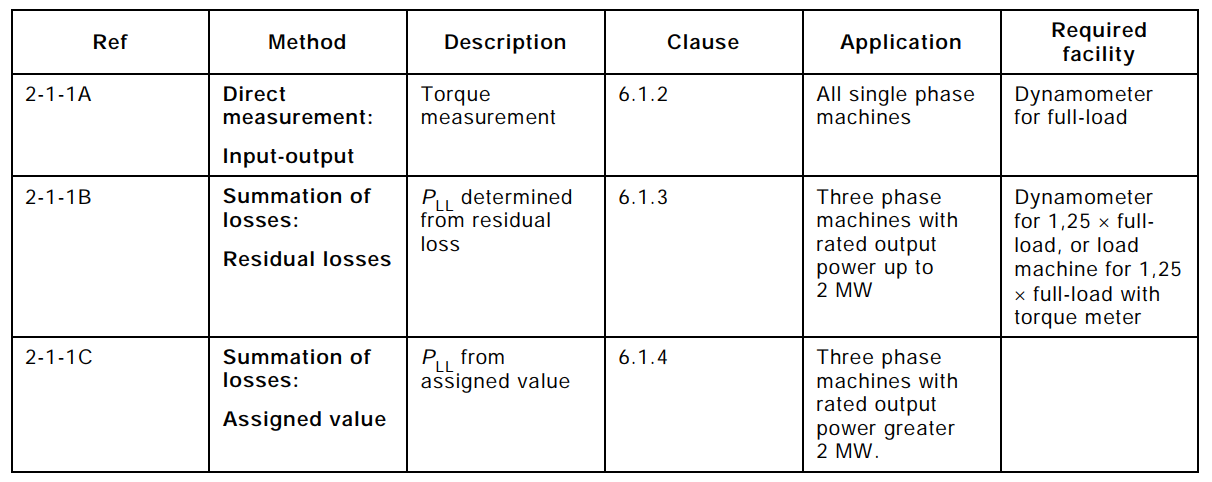
\includegraphics[width = 5.5in]{./Figures/MS/23.png}
		\rule{35em}{0.5pt}
	\caption{Preferred testing methods defined by IEC 60034-2-1:2014}
	\label{fig:Preferred testing methods defined by IEC 60034-2-1:2014}
\end{figure}
\begin{figure}[htbp]
	\centering
		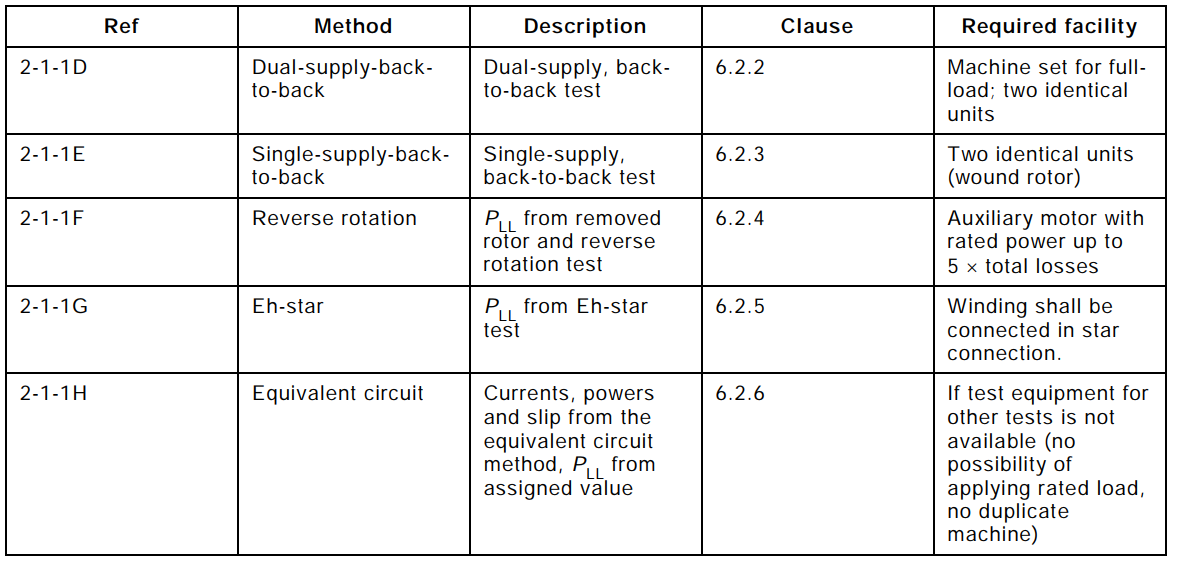
\includegraphics[width = 5.5in]{./Figures/MS/24.png}
		\rule{35em}{0.5pt}
	\caption{Routine/Field testing methods defined by IEC 60034-2-1:2014}
	\label{fig:Routine/Field testing methods defined by IEC 60034-2-1:2014}
\end{figure}

\subsection{Testing methods with pumps}
Testing of pumps is done under ISO-9906 standard which provides conditions and requirements for testing of pumps. The following table shows the accuracy of pump testing:
\begin{figure}[htbp]
	\centering
		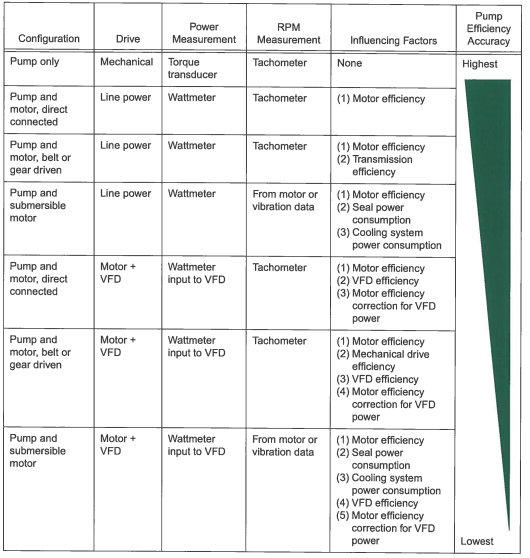
\includegraphics[width = 5.5in]{./Figures/MS/25.png}
		\rule{35em}{0.5pt}
	\caption{Testing Accuracy by configuration defined by ISO-9906\cite{iso9906}}
	\label{fig:Testing Accuracy by configuration defined by ISO-9906}
\end{figure}
This table shows that the best accuracy is achieved in the case of separate testing of pumps and motors. So, IEC 60034-2-1 was used for testing the motors separately. % What to Write 
% % Chapter 1
\setstretch{1.8}
\chapter{The Experimental Setup} % Write in your own chapter title
\label{Chapter3}
\lhead{Chapter 3. \emph{The Experimental Setup}} % Write in your own chapter title to set the page header

\section{Introduction}

This chapter describes the experimental setups created for the test bench. The schematics were created and tested in Simulink and run using MATLAB scripts. Since this project aims to develop testing methods for motors that are to be used in the lab, direct methods for efficiency determination have been used as they provide much more accurate results. The basic component that differentiates the setups from each other is the implementation of the dynamometer, i.e. the loading device. 

\section{Software Environment}
This section describes the details of software, libraries and parts used in creating the experimental setups. Simulink was used to create the simulations. Simulink is created by Mathworks and comes as a part of MATLAB. MATLAB R2019a was used for this project. Simulink is a graphical programming environment for modeling, simulating and analyzing a variety of different setups and is extensively used in industry because of its ability to create production level embedded codes using its embedded coder. For this project, the Simscape PS(Physical Systems) library was used, which is a relatively new addition to Simulink and provides a very accurate simulation of physical systems of multiple domains, including electrical, rotational mechanical, translational mechanical, thermal, etc., and providing a color scheming to separate each types of system from the other. 

\begin{figure}[htbp]
	\centering
		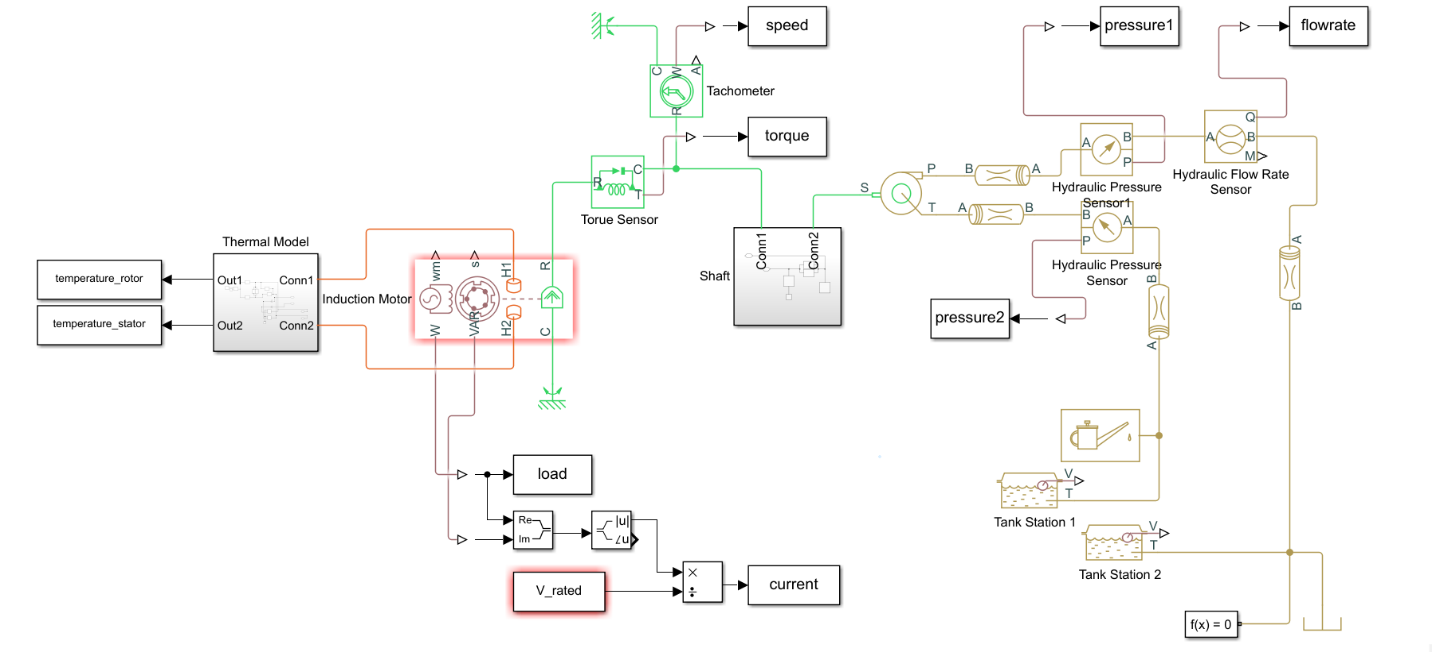
\includegraphics[width = 4.5in]{./Figures/MS/fig31.png}
		\rule{35em}{0.5pt}
	\caption{Example of a motor-pump system in Simulink}
	\label{fig:Example of a motor-pump system in Simulink}
\end{figure}
The figure above shows rotational mechanical(green), and hydraulic(brown) systems, used to create a test bench for testing a centrifugal pump attached to an induction motor. 
\begin{figure}[htbp]
	\centering
		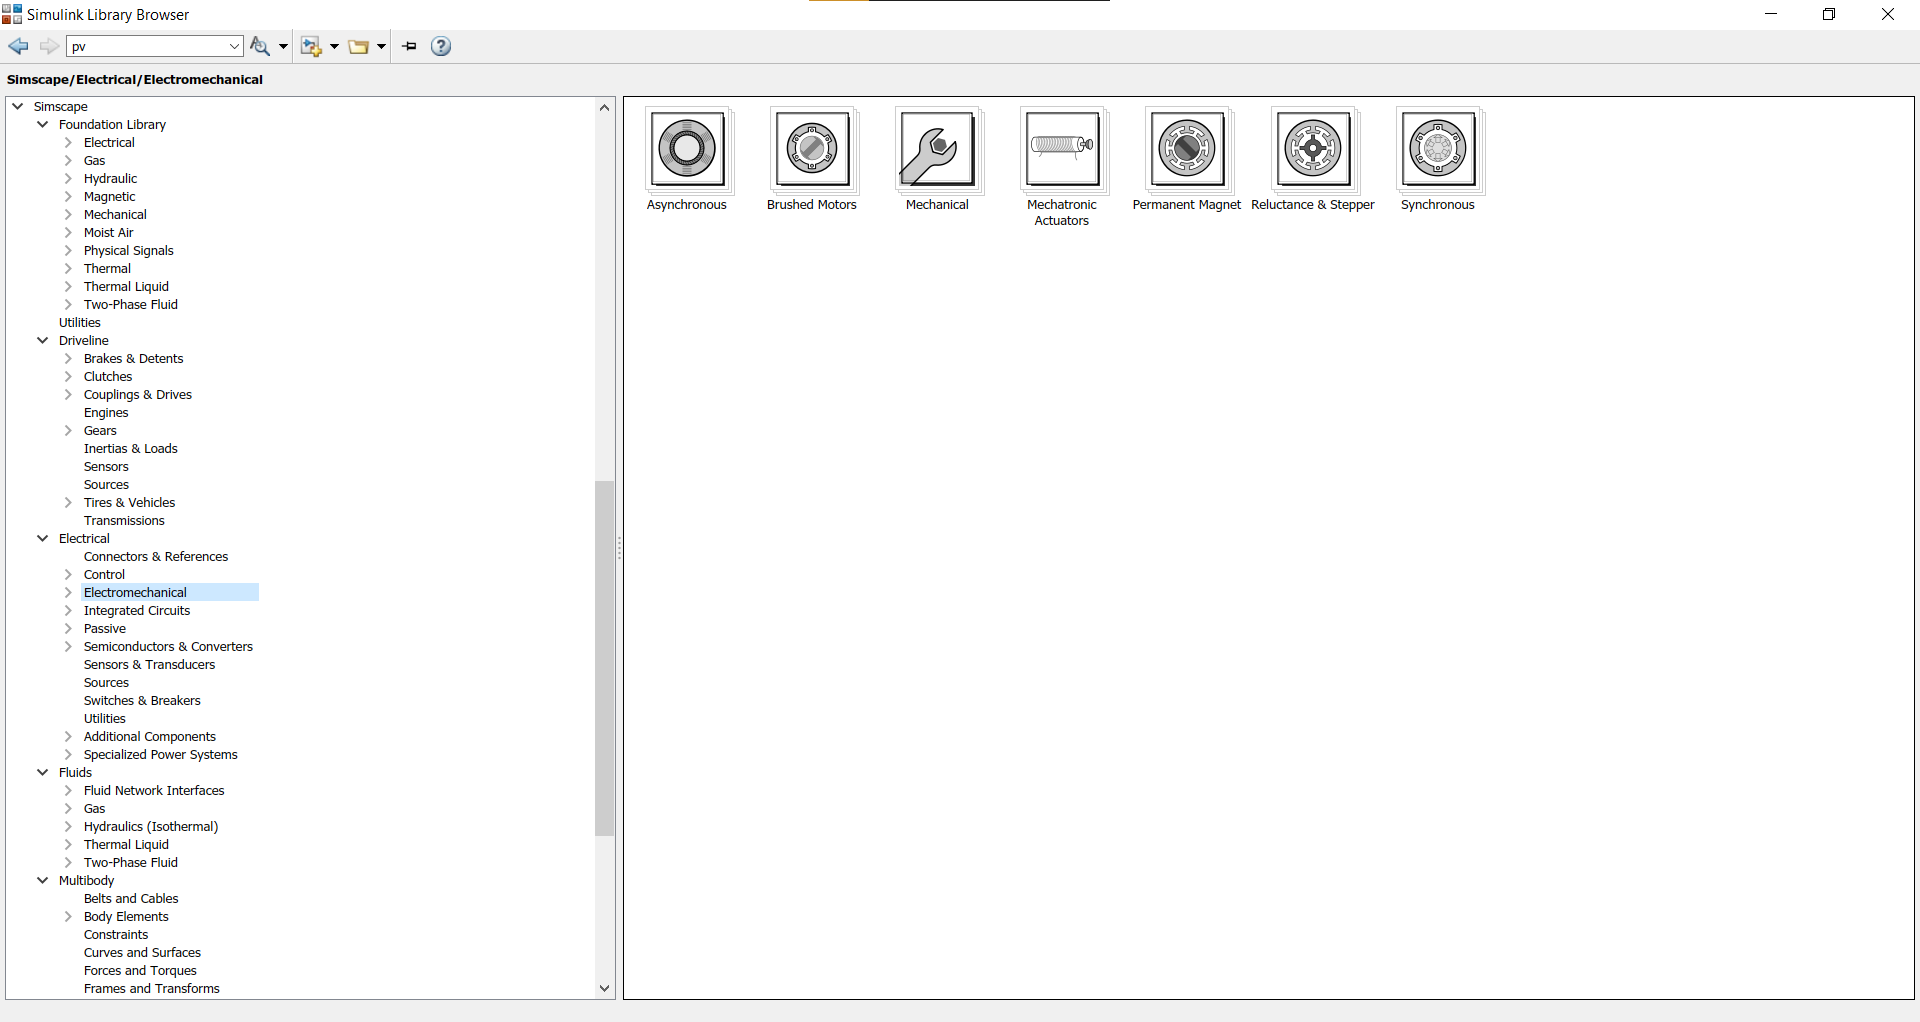
\includegraphics[width = 4.5in]{./Figures/MS/fig32.png}
		\rule{35em}{0.5pt}
	\caption{Simscape library in Simulink}
	\label{fig:Simscape library in Simulink}
\end{figure}
The above figure provides an overview of the variety of systems provided by Simscape. 
After the setups were created, MATLAB scripts were used to call these and run the tests under the conditions and requirements provided by the IEC standard. MATLAB provides a sim() function to call simulations from within a script and the ‘to workspace’ blocks in Simulink transfer the data between the two environments.

\section{Control Scheme}
PID control is used to control the loading of motors. PID is s simple, yet widely used control technique in closed loop systems. It takes error as input, and 3 parameters, proportional gain(K\textsubscript{p}), integral gain(K\textsubscript{i}) and proportional gain(K\textsubscript{d}), that are multiplied by the error, its integral and derivative respectively, and then added together to provide a control signal to run the system at the desired setpoint, as shown in the figure below:
\begin{figure}[htbp]
	\centering
		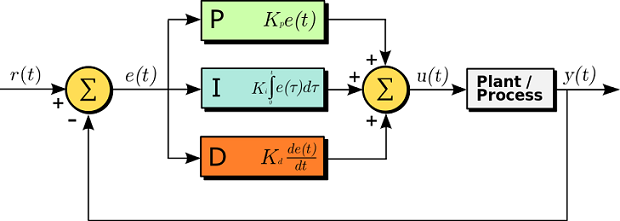
\includegraphics[width = 4.5in]{./Figures/MS/fig317.png}
		\rule{35em}{0.5pt}
	\caption{Block diagram of PID control.}
	\label{fig:Block diagram of PID control.}
\end{figure}
The equation for the PID control is:
\begin{equation}
	U(t) = K_p e(t) + K_i \int\limits_{t=0}^{\infty} e(t) d(t) + K_d \frac{de(t)}{dt}
\end{equation}
While for embedded systems, the equation is written in discrete time domain as:
U(k) = kp e(k) + ki sum(lim k=0 to k-1)e(i) + ki e(k) + kd(e(k) – e(k-1))
\begin{equation}
	U(k)=K_p e(k) + K_i \sum\limits_{i=0}^{k-1}e(i) + K_i e(k) + K_d(e(k) - e(k-1))
\end{equation}

For the project at hand, the output mechanical load of the motor was to be set. The following figure shows how the mechanical load was calculated and fed to PID controller:
\begin{figure}[htbp]
	\centering
		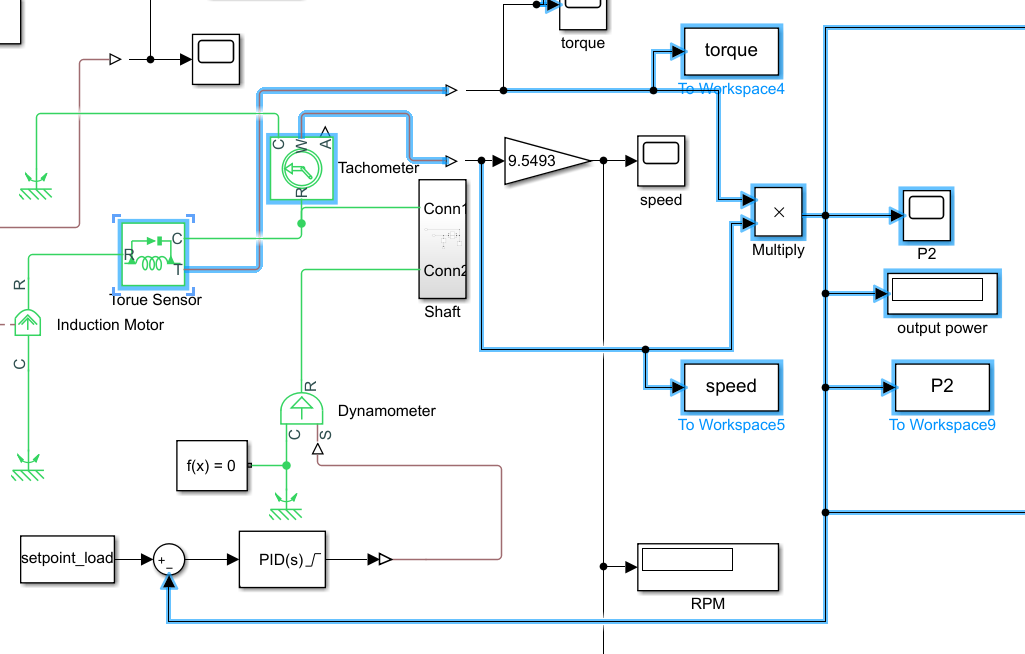
\includegraphics[width = 4.5in]{./Figures/MS/fig318.png}
		\rule{35em}{0.5pt}
	\caption{PID control block in Simulink}
	\label{fig:PID control block in Simulink}
\end{figure}

The output power was calculated from the product of torque and angular speed from their respective sensors, and the multiplied and fed to the PID controller. The setpoint\_load variable comes from the matlab workspace from where the simulations were called.
The Simulink PID block provides an automated tuning option. The Transfer function based tuning method was used to tune the PID controllers.

\begin{figure}[htbp]
	\centering
		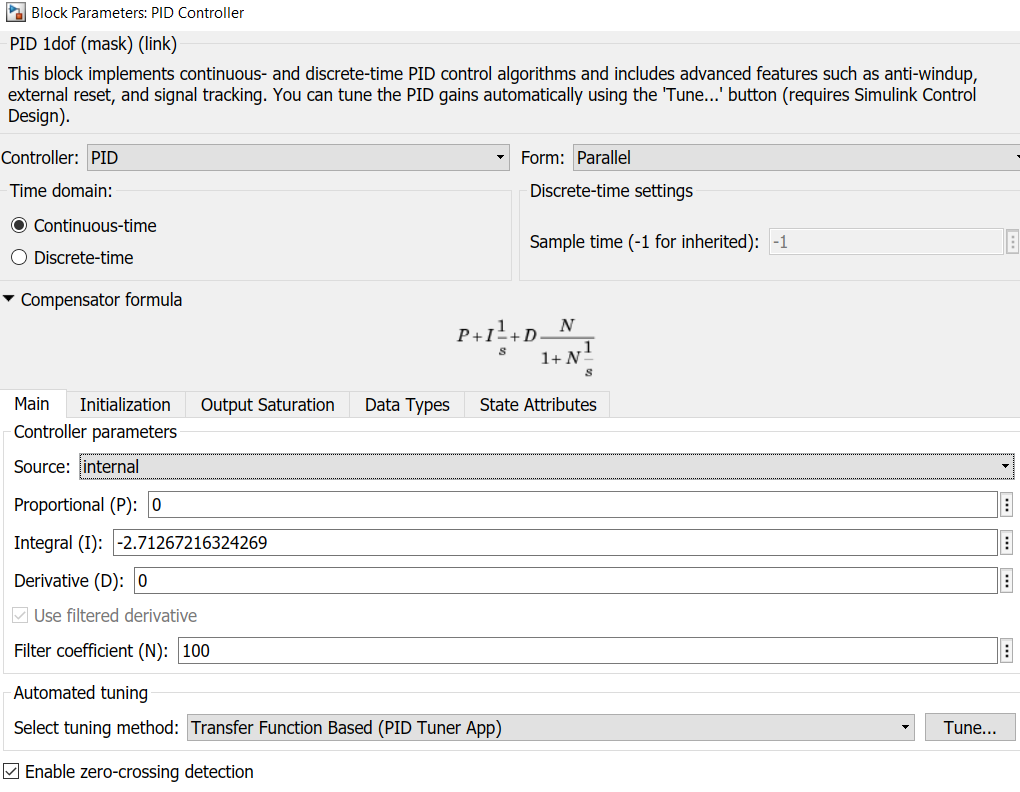
\includegraphics[width = 4.5in]{./Figures/MS/fig319.png}
		\rule{35em}{0.5pt}
	\caption{PID parameters overview in Simulink}
	\label{fig:PID parameters overview in Simulink}
\end{figure}

\begin{figure}[htbp]
	\centering
		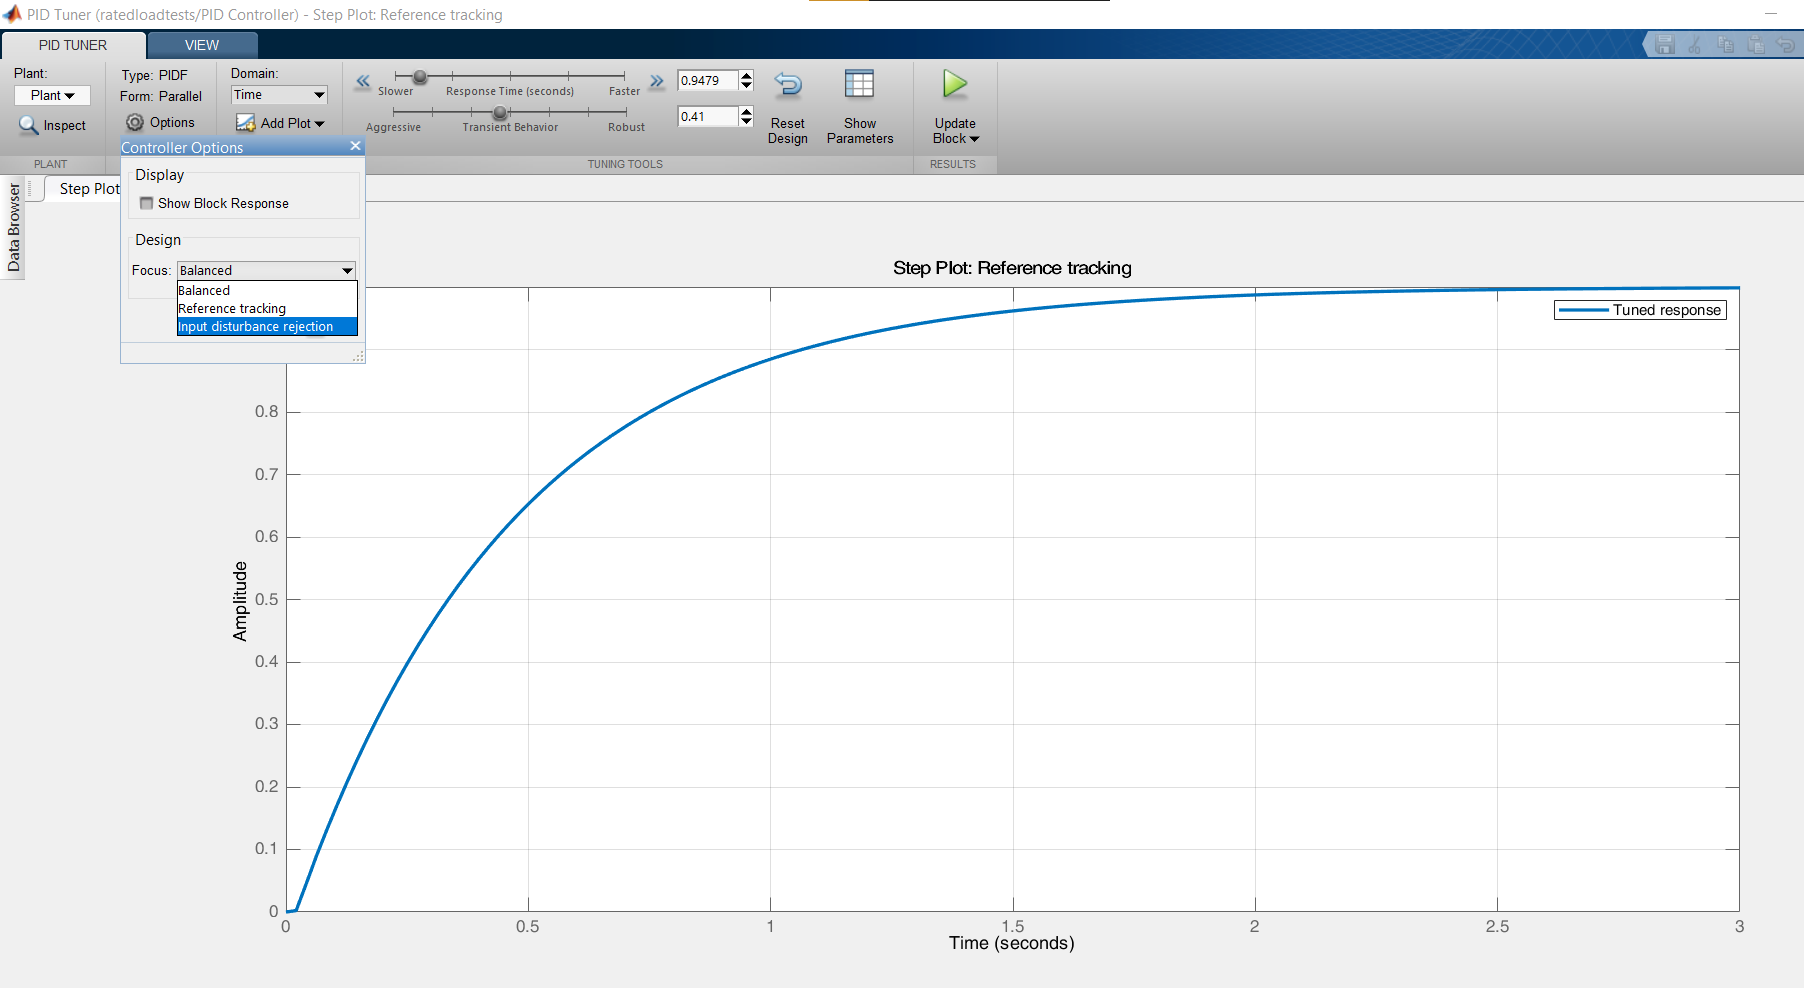
\includegraphics[width = 4.5in]{./Figures/MS/fig320.png}
		\rule{35em}{0.5pt}
	\caption{PID auto-tuner in Simulink}
	\label{fig:PID auto-tuner in Simulink}
\end{figure}
The PID tuner app provides us with tuning tools to allow us change and visualize the step response of the system, so the tuning in the app is quite interactive, and has been proven to be quite useful for tuning actual systems as well, by building the systems in Simulink and using the tuning app.

\section{Adaptions for load control}
As described above, a motor testing involves loading a motor with different amounts of loads and observing the quantities such as current, voltage, frequency, temperature, speed, torque, etc. So to create a testing setup for a motor, we need to have some sort of technique of controlling the load on a motor, where the load is the mechanical load on the shaft, since a motor outputs rotational kinetic energy. 
\begin{figure}[htbp]
	\centering
		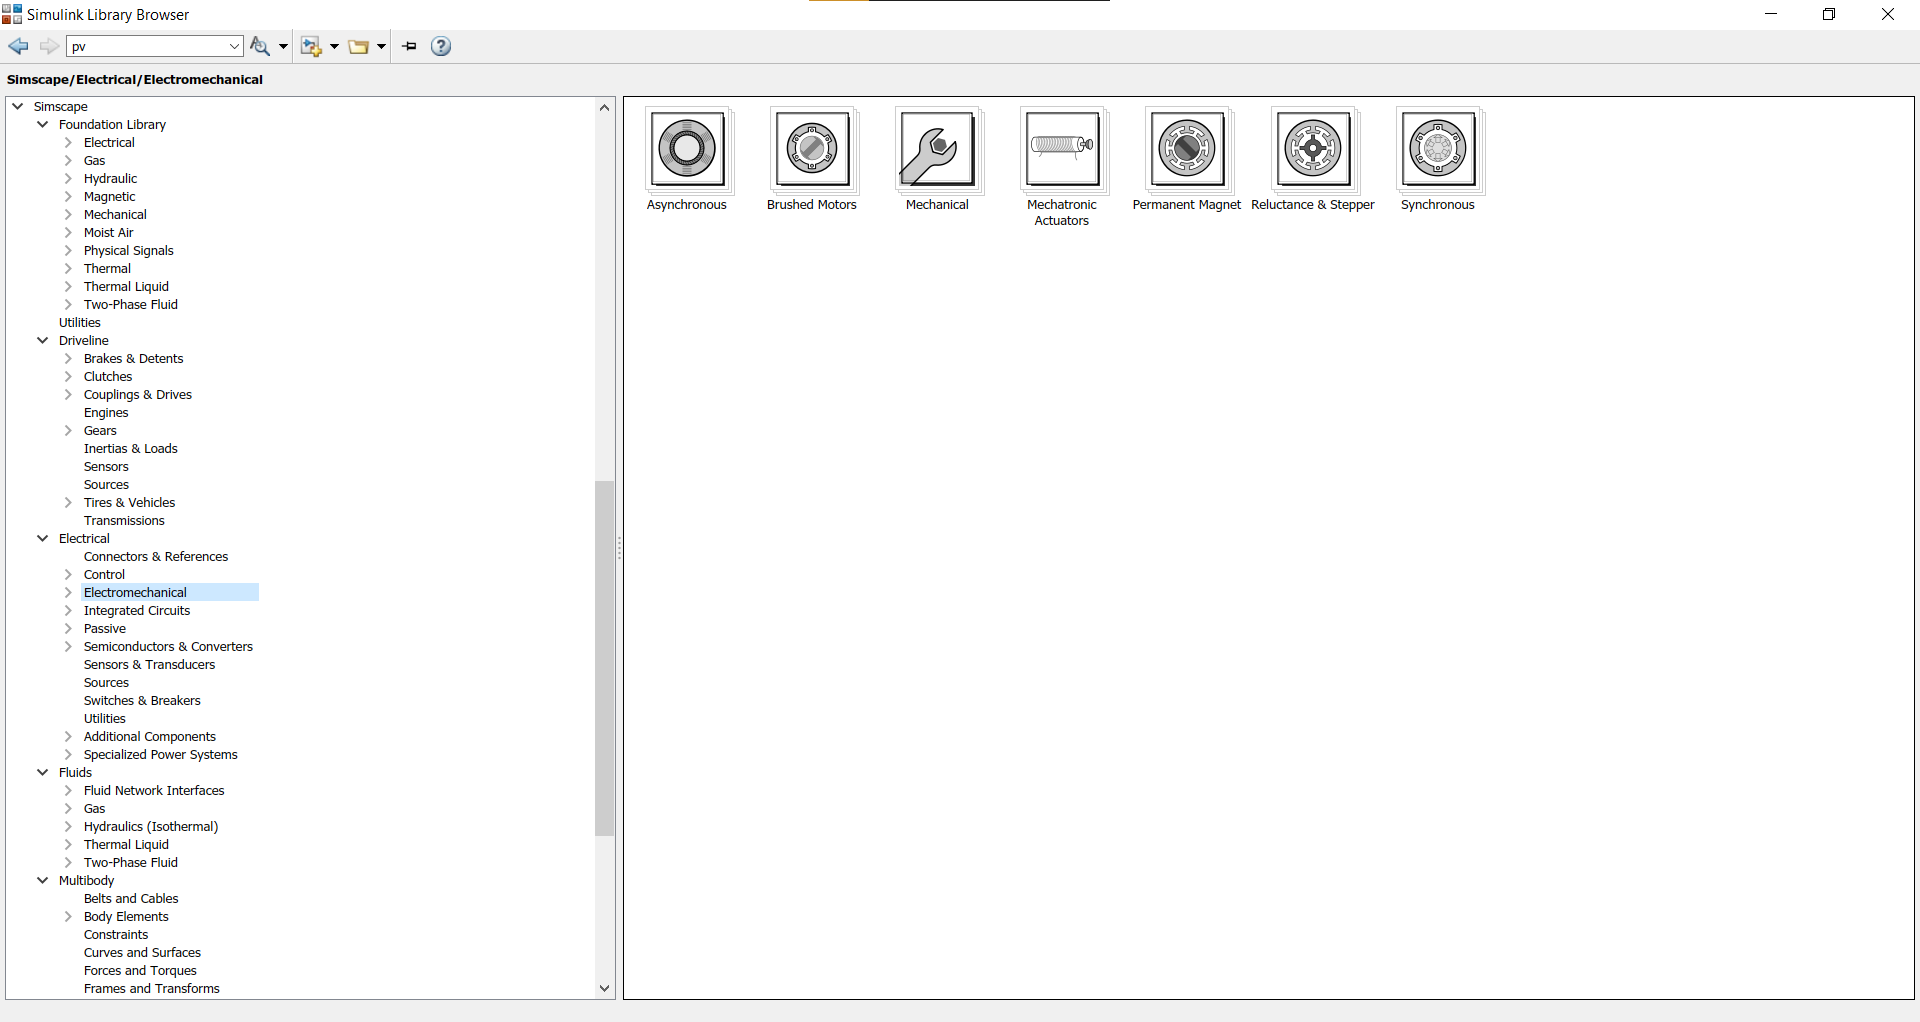
\includegraphics[width = 4.5in]{./Figures/MS/fig32.png}
		\rule{35em}{0.5pt}
	\caption{Block diagram of system to be implemented}
	\label{fig:Block diagram of system to be implemented}
\end{figure}

\subsection{Generic Test bench in Simulink}
\begin{figure}[htbp]
	\centering
		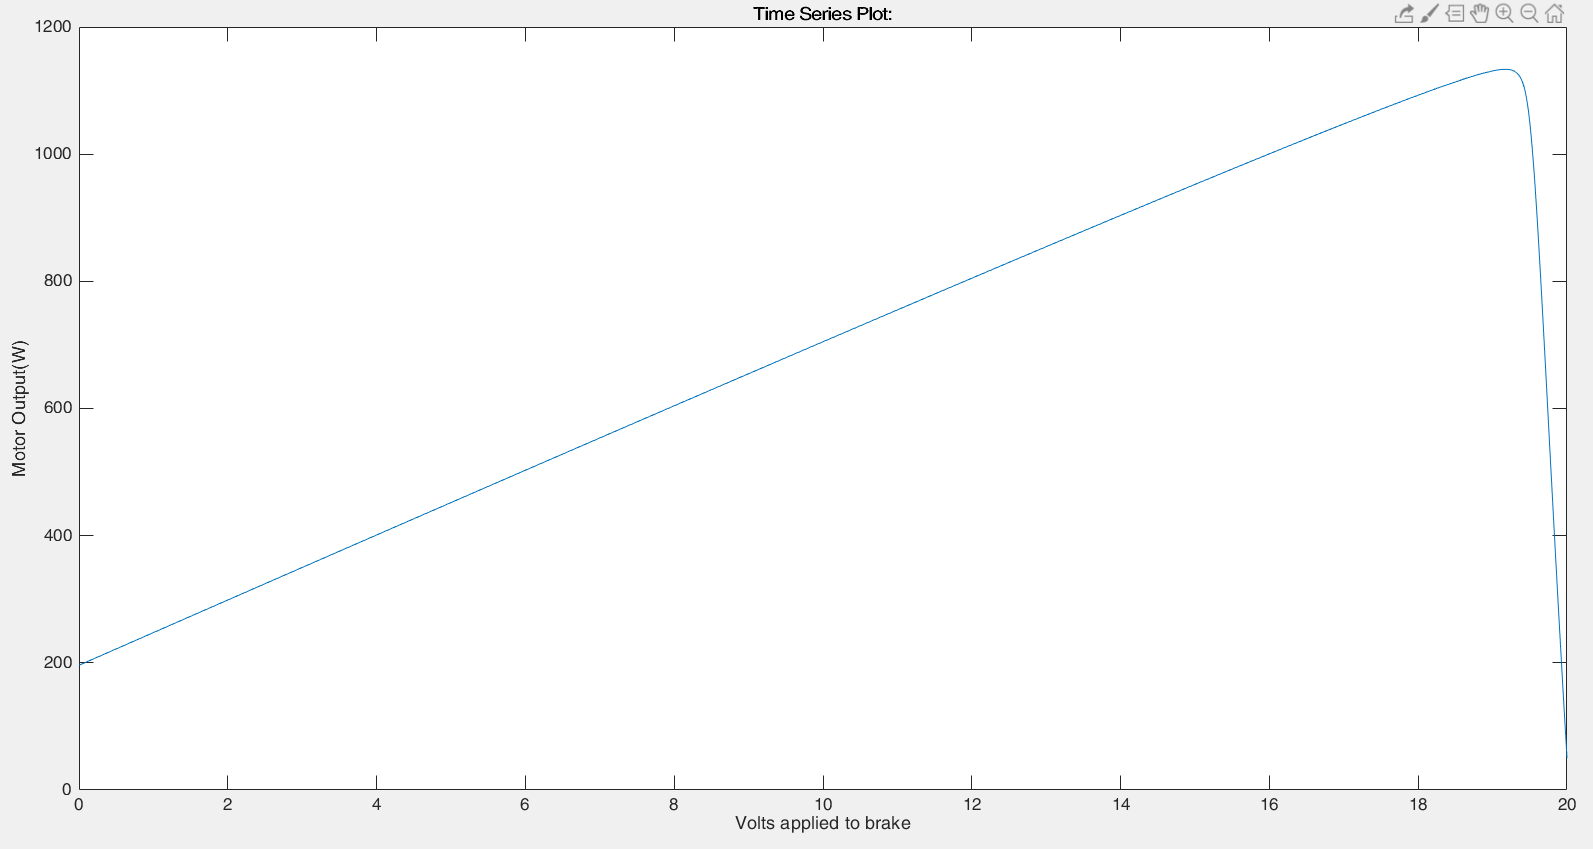
\includegraphics[width = 4.5in]{./Figures/MS/fig322.png}
		\rule{35em}{0.5pt}
	\caption{Generic Test bench in Simulink}
	\label{fig:Generic Test bench in Simulink}
\end{figure}
T¬he above figure shows a generic testbench designed in Simulink. A generic dynamometer block has been selected as the load and the different measurement systems have been highlighted. The measurements are taken using ‘to workspace’ blocks, which take measurements in the form of a MATLAB timeseries object and send it the to workspace, so they can be used by the scripts. Such a simulation can be called using the sim(model,time) command in matlab scripts. Apart from that, there are also some PS-to-simulink conversion blocks which convert the physical measurements, shown by brown lines to Simulink generic signals, shown by black lines. The selected motor model has a supply builtin, as is clear from its diagram, and more details on how electrical quantities are being measure are shown in the subsequent sections. Unlike the electrical system, the mechanical and thermal systems are visible as green and orange components and lines respectively. The selection of Simscape also had an advantage over the powersim library, as the powersim library is quite old and also doesn’t deal with the thermal aspects of the motors. The details for thermal and mechanical measurements are also discussed later in this chapter. Now that a base template for motor test benches has been developed, it can be extended further using different implementations of the dynamometers. The scripts used to call these simulations are discussed in the next chapter. Following are the two dynamometer implementations used for this project. Two general schemes of controlling the loading have been adapted, and multiple adaptions for both have been tested.

\subsection{Coupling a generator with the motor and controlling its electrical load}
In this method, the shaft of the motor is coupled to another machine that will work as a generator, and by controlling the load connected to the generator, the loading of the motor can be controlled. A DC machine is used as a generator in this case as controlling DC load using electronics is much easier, linear and cost effective as compared to ac. In such setups, a rheostat is connected to the generator so that the load can be controlled, smoothly and easily. In the current setup, this rheostat needs to be replaced by an electronic device, so that the it can be controlled easily using an embedded system. A voltage controlled current source(VCCS) or Voltage Controlled Resistor(VCR) scheme needs to be applied and FETs are the most fit device for this purpose. The dc machine is coupled to load and an FET which controls the current through the load, providing a variable load with multiple settings. The following figure shows the load created by such method:
\begin{figure}[htbp]
	\centering
		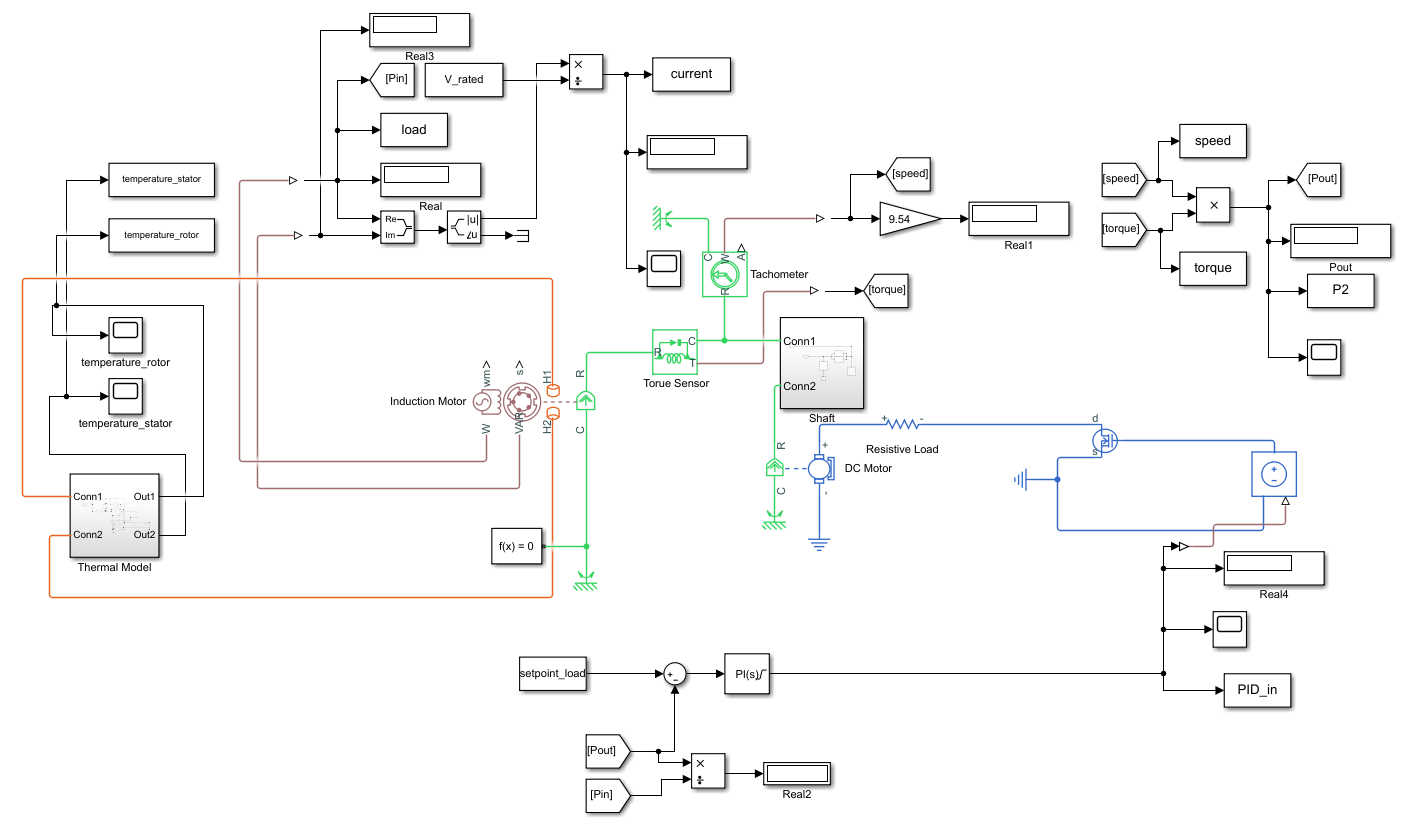
\includegraphics[width = 4.5in]{./Figures/MS/fig34.png}
		\rule{35em}{0.5pt}
	\caption{Testbench implementation using resistive load control by FET}
	\label{fig:Testbench implementation using resistive load control by FET}
\end{figure}
This method is similar to the manual testing method of motors where the motor is coupled to another machine that will act as a generator connected with a rheostat. As the load is increased by moving the rheostat slider, the torque on the motor is increased and hence, the motor can be tested at multiple load points. What the first method has implemented is, the rheostat is now replaced by a resistance and a power-FET. By controlling the gate voltage, the current through the resistance can be controlled, which in turn controls the torque on the motor. This can be implemented by two control methods using an embedded device:
\begin{itemize}
	\item DAC (Digital to analog converter)
	\item PWM (Pulse Width Modulation)
\end{itemize}
The DAC control requires a large linear control region for the FET device, so a JFET is better for the case, when a DAC is used to control the load while in case of PWM, pulses of variable duty cycle are applied to the load to control the current flow, so a MOSFET is the better choice. In both methods, a PID controller can be used easily to control the system. In case of PWM, the switching frequency should be set high to remove noise and such that the switching frequency is much higher than the motor response so that the electromechanical conversion is low-passed, and the torque and speed remain smooth. This is a problem for small, responsive motors, where the frequency needs to be set much higher, while it is not much of an issue for large motors. 
\begin{figure}[htbp]
	\centering
		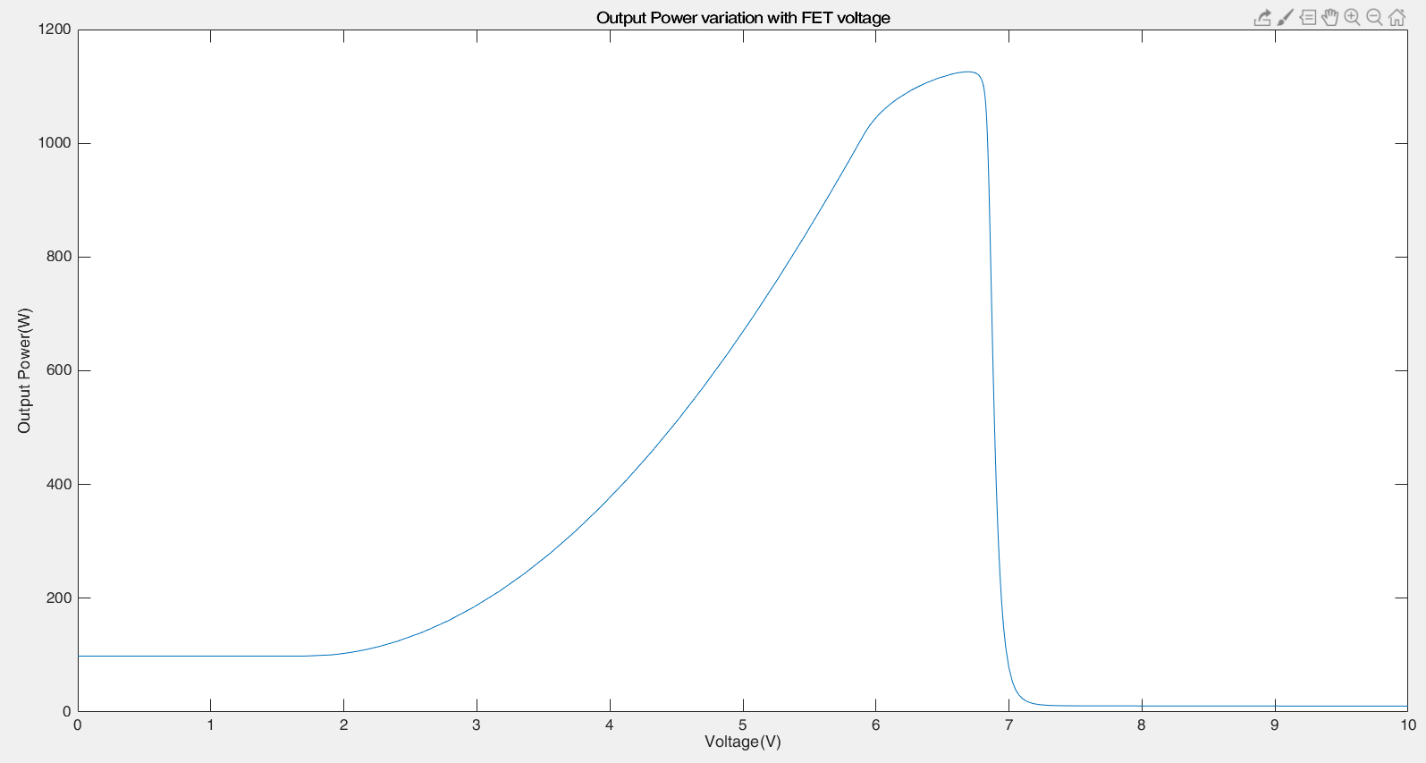
\includegraphics[width = 4.5in]{./Figures/MS/fig35.png}
		\rule{35em}{0.5pt}
	\caption{Relation between FET gate voltage and output power for a 1hp motor}
	\label{fig:Relation between FET gate voltage and output power for a 1hp motor}
\end{figure}
The above figure shows the controllable output power region vs the voltage applied on the FET during the simulation. After a voltage of 7V, the loading was above the motor max, and hence the motor went to a stall, reducing the output power(speed * torque) to almost zero.

\subsection{Using Electronic Controlled Brakes}
There are three common types of brakes that can be controlled electronically or electrically. 
\begin{itemize}
	\item	Magnetic particle brakes
	\item	Servo Brakes
	\item	Eddy current brakes
\end{itemize}
Magnetic particle brakes contain a fine-grained magnetic material and pads with holes in them. When a signal is applied to the terminals, the particles start filling the holes, and pressing the pads against the disc, proportional to the applied voltage. Magnetic particle brakes are a relatively new type of electronic brakes and are being used in small autonomous vehicles.
Eddy current brakes are electrically controlled, using an AC voltage. In these brakes, a conductive disk, mounted on the shaft, is placed in an electromagnet, and when the magnets are powered on and the disk rotates, an eddy current is induced proportional to the applied power, which produces some power, that is dissipated through the disk, to provide a braking torque force.  A major problem with eddy current brake is that it doesn’t have a holding torque. Therefore, it has to be used with standard mechanical brakes.
Servo brakes are electronically controlled, and it contains a servo motor, which controls the position of the brake pads on the disk. 
For this setup, Magnetic particle brakes have been selected, shown in the following figure:
\begin{figure}[htbp]
	\centering
		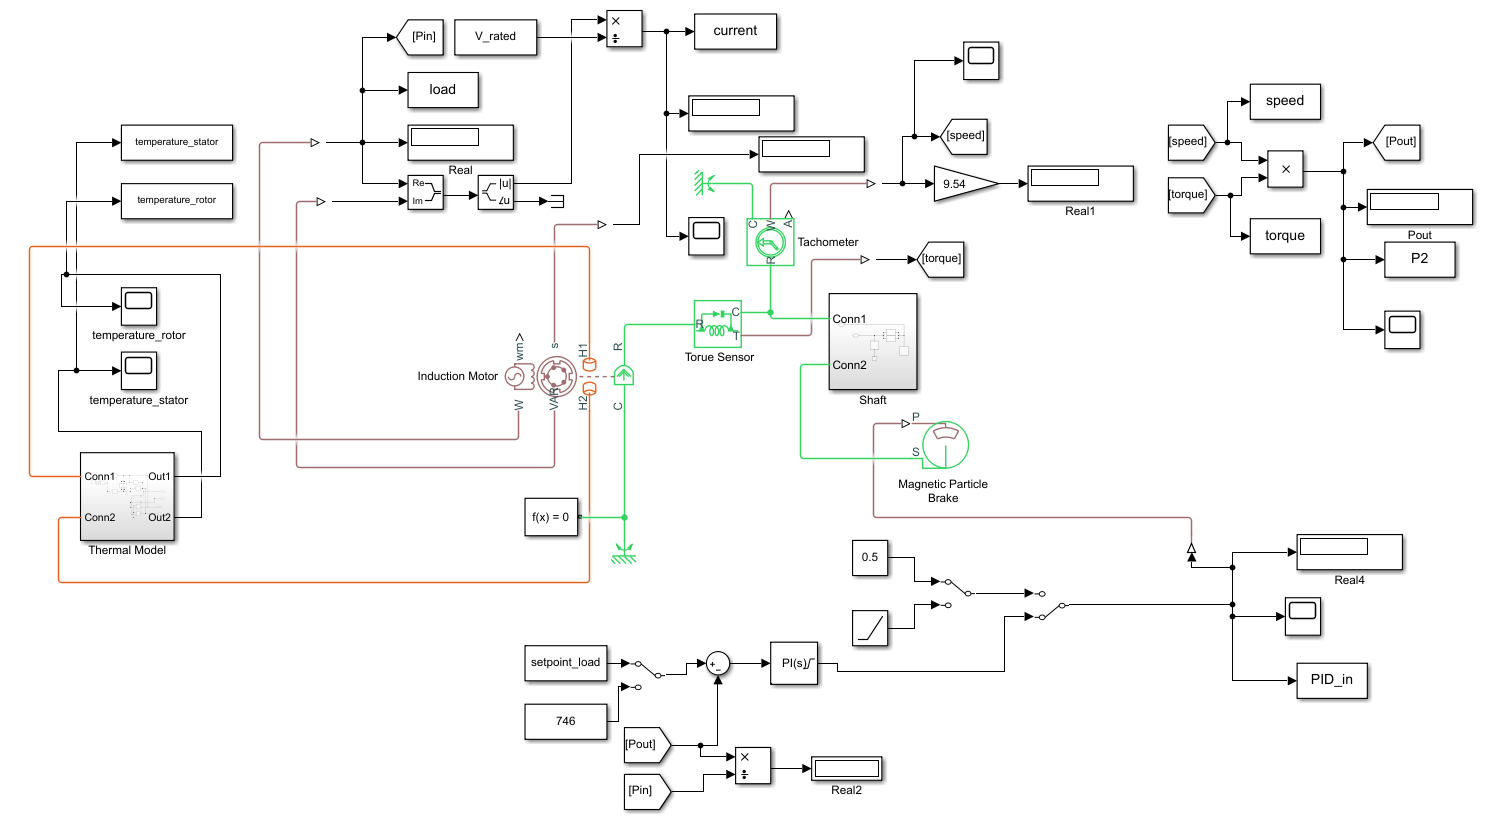
\includegraphics[width = 4.5in]{./Figures/MS/fig321.png}
		\rule{35em}{0.5pt}
	\caption{Motor linked with a brake in Simulink}
	\label{fig:Motor linked with a brake in Simulink}
\end{figure}
The brakes available in simulink are only mechanical brakes, but the particle brake is controlled in a similar fashion, i.e. a voltage applied as the control signal, which is a generic Simulink signal applied to the brake on port P, which will be referred to as voltage in the scope of this document.

The following graphs show the relation between applied voltage on the brake and input/output power of the motor.
\begin{figure}[htbp]
	\centering
		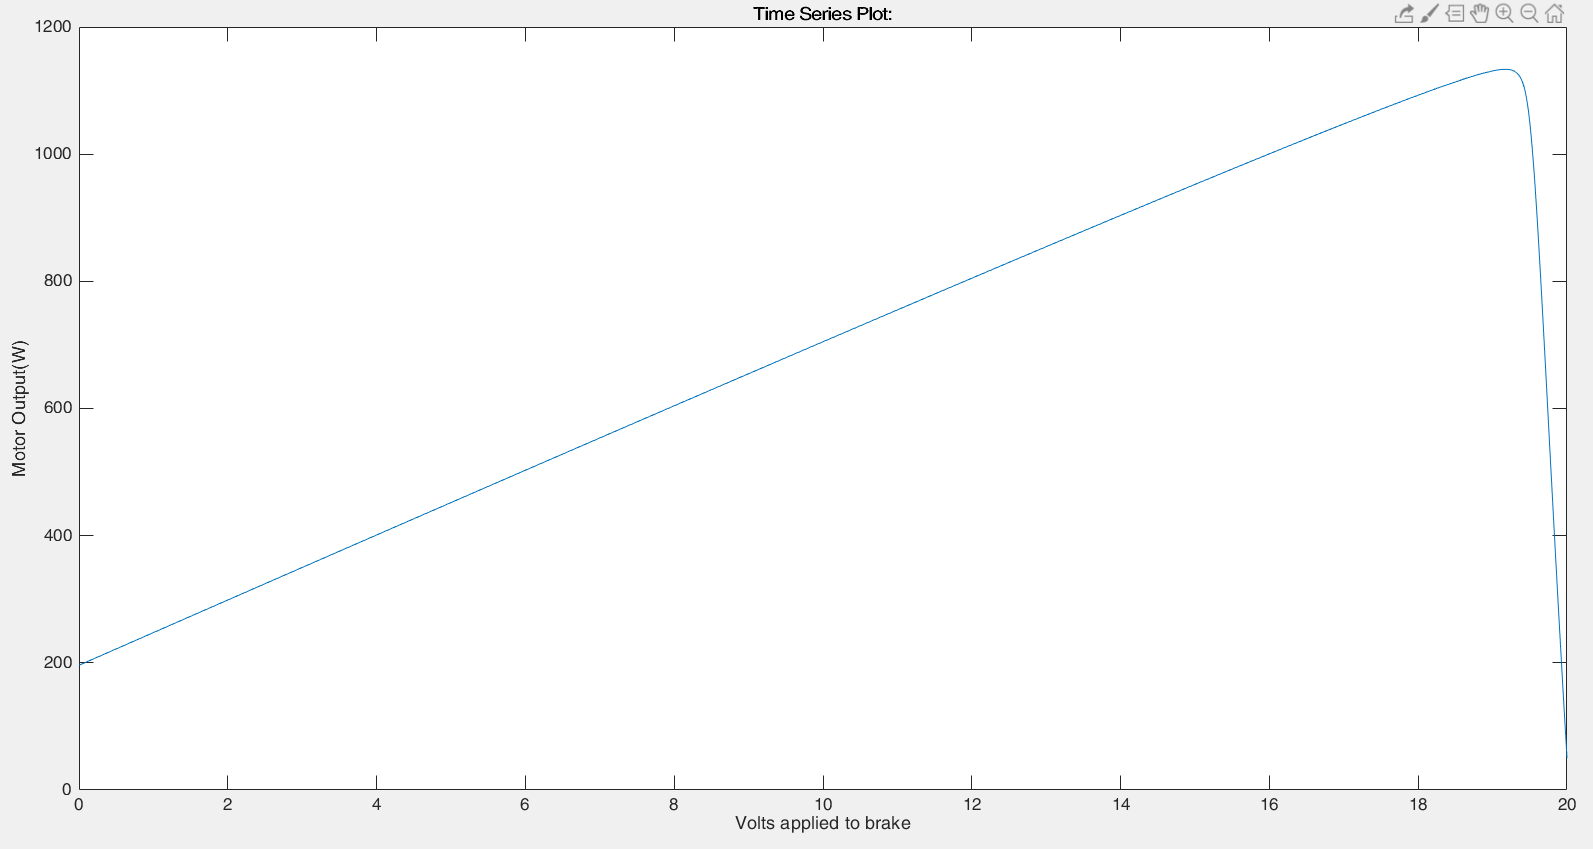
\includegraphics[width = 4.5in]{./Figures/MS/fig322.png}
		\rule{35em}{0.5pt}
	\caption{Relation between brake voltage and output power for a 1hp motor}
	\label{fig:Relation between brake voltage and output power for a 1hp motor}
\end{figure}
\begin{figure}[htbp]
	\centering
		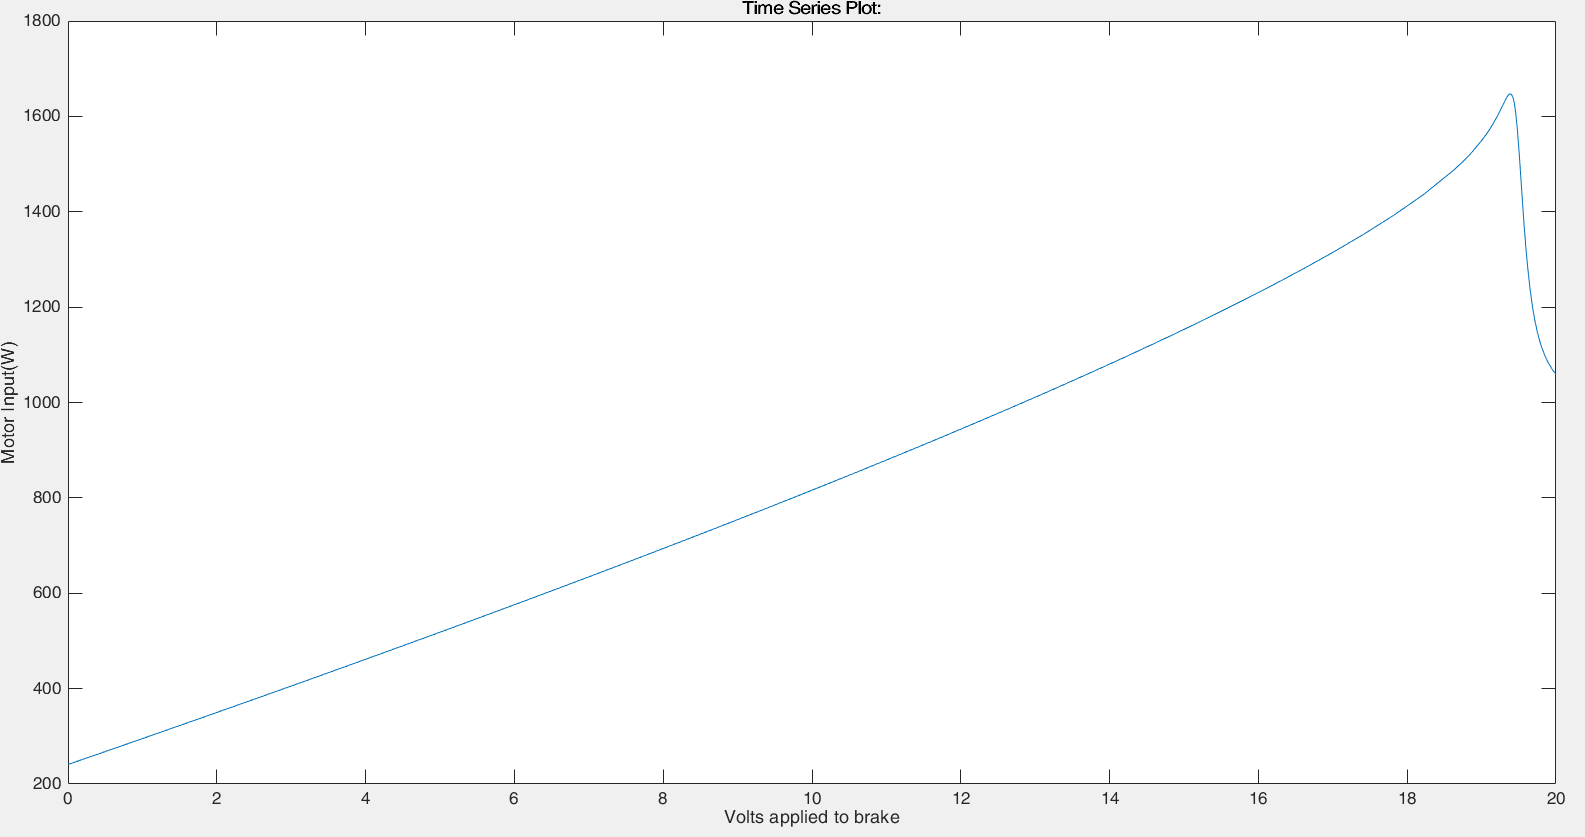
\includegraphics[width = 4.5in]{./Figures/MS/fig323.png}
		\rule{35em}{0.5pt}
	\caption{Relation between brake voltage and input power for a 1hp motor}
	\label{fig:Relation between brake voltage and input power for a 1hp motor}
\end{figure}


\section{Instrumentation}
The quantities that were required to be measured by IEC are:
\begin{itemize}
	\item	Input Power
	\item	Torque
	\item	Current 
	\item	Voltage
	\item	Frequency
	\item	Angular speed
	\item	Coolant temperature (if applicable)
	\item	Winding temperature
	\item	Winding Resistance
\end{itemize}

\subsection{Measurement of electrical quantities}
The following rules are defined for the operating conditions:
\begin{itemize}
	\item Voltage: IEC-60034-1, clause 7.2.1.1 defines that AC motors supplied by an AC generator power supply of nearly fixed freqency shall be appropriate for the testing on a voltage source having a harmonic voltage factor(HVF) not surpassing 2\% for single phase and three phase motors, calculated from the following equation:

\begin{equation}
HVF=\sqrt{\sum\limits_{n=1}^k\frac{u_{n}^2}{n}}
\end{equation}
\begin{align*}
\text{where:}\quad
 u\textsubscript{n}     &=  \text{ratio of harmonic voltage U\textsubscript{n} to the rated voltage U\textsubscript{N}} \\
 n     					&=  \text{order of the harmonic} \\   
 k 						&=  \text{13}
\end{align*}

	\item	IEC-60034-1, clause 7.2.1.1 defines that during all tests, the mean supply frequency should remain within 0.1\% of the required, for the tests being performed
\end{itemize}

For measuring instrument uncertainties, IEC recommends using digital instruments whenever feasible. From IEC-60034-2-1, clause 5.5.2, the measuring instruments need to have an accuracy class of 0.2 or equivalent for when direct tests are being performed and 0.5 in the cases when indirect tests are performed according to IEC 60051. The measuring apparatus should include errors of transformers and transducers, if being used and should reach a max uncertainty of 0.2\% of reading at power factor 1.0
 
\subsection{Measurement of mechanical quantities}

\subsubsection{Torque}
IEC-60034-2-1, clause 5.5.3 defines that the sensors used to calculate torque should have a minimum class of 0.2. The lowest torque to be measured should be atleast 10\% of the torque meter's rated torque. For better class equipement, the allowed limits for torque can be adjusted as required.

\begin{figure}[htbp]
	\centering
		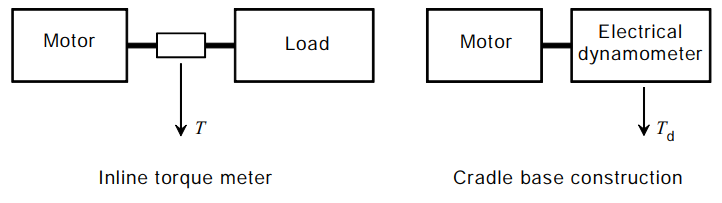
\includegraphics[width = 4.5in]{./Figures/MS/fig36.png}
		\rule{35em}{0.5pt}
	\caption{Types of torque sensors from IEC-60034-2-1}
	\label{fig:Types of torque sensors from IEC-60034-2-1} 
\end{figure}

When a cradle base construction dynamometer is used to measure the shaft torque, a torque correction test must be performed to offset the friction losses in the bearings of the dynamometer. The machine torque T is calculated using the formula:
\begin{equation}
T=T_{d}+T_{c}
\end{equation}
It should be observed that the temperature of the torque sensor, i.e. in the vicinity of the rotor, may be greater than the ambient temperature and is known to have a substantial impact to total uncertainty. Therefore, the impact of temperature to the uncertainty should be restricted to 0.15 \% of full scale. If that is not feasible, a suitable temperature correction has to be applied. Parasitic loads should be lessened by shaft alignment and the use of flexible couplings.

\subsubsection{Speed}
IEC-60034-2-1, clause 5.5.4 defines that the instruments used to determine supply frequency shall have an accuracy of 0.1 \% of full scale. The speed measurement should be accurate within 0.1 rpm.

\subsection{Measurement of thermal quantities}
IEC-60034-2-1, clause 5.5.4 states that the instruments used to determine temperatures shall have an accuracy of 1 K. 
From From IEC-60034-2-1, clause 5.7.2, The winding temperature shall be calculated by one of the following methods:
\begin{itemize}
	\item Temperature determined from the rated load test resistance RN by the extrapolation method as defined in 5.7.1(Note: Motors that are to be tested for regulatory purposes must not be disassembled. Therefore, measurement of winding temperature shall be using change of resistance method.)
	\item Temperature measured directly by either ETD or thermocouple.
	\item Temperature determined according to 1 on an identical machine of the same construction and electrical design.
	\item When load capability is unavailable, calculate temperature according to IEC 60034-29.
	\item When the rated load test resistance cannot be measured directly, the winding temperature shall be presumed to be the same as the reference temperature of the rated thermal class as given in the following table:
\end{itemize}
\begin{figure}[htbp]
	\centering
		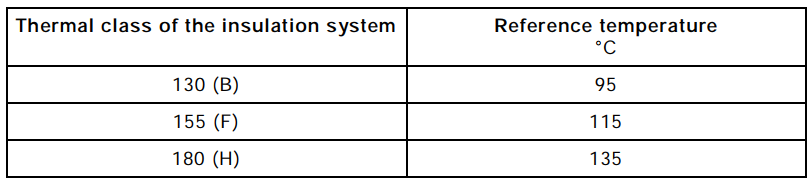
\includegraphics[width = 4.5in]{./Figures/MS/fig310.png}
		\rule{35em}{0.5pt}
	\caption{Table of thermal class insulation and their reference temperature from IEC-60034-2-1}
	\label{fig:Table of thermal class insulation and their reference temperature from IEC-60034-2-1} 
\end{figure}


If the rated temperature rises or the rated temperature is specified as that of a lower thermal class than that used in the assembly, the reference temperature shall be that of the lower thermal class. When necessary, the winding resistance values recorded through test shall be described by a standard reference temperature of 25 \textdegree C. The correction factor to fine-tune the winding resistance (and the slip in the case of cage induction machines) to a standard reference coolant temperature of 25 \textdegree C shall be determined by:


\begin{equation}
k_{\theta}=\frac{235+\theta_{w}+25-\theta_{c}}{235+\theta_{w}}
\end{equation}
\begin{align*}
\text{where:}\quad
 k\theta    &=  \text{is the temperature correction factor for windings.} \\
 \theta\textsubscript{w}     &=  \text{is the winding temperature according to 5.7.2} 	   \\   
 \theta\textsubscript{c} 	 &=  \text{is the inlet coolant temperature during test.}
\end{align*}

The temperature constant 235 is for copper; this should be interchanged by 225 for aluminum conductors. For machines with water as the primary or secondary coolant, the water reference temperature shall be 25 \degree C according to Table 4 of IEC 60034-1:2010. Substitute values may be specified by agreement.		

\subsection{Units of measurements}
From IEC-60034-2-1, clause 5.5.6, Unless otherwise specified, the units of values are SI-units as listed in IEC 60027-1.

\subsection{State of the machine under test and test categories}
Tests must be performed on a connected machine with the necessary elements in position, to achieve test conditions equal or very similar to normal operating conditions.
Note 1: It is better that the machine be chosen arbitrarily from series production without particular considerations.
Externally approachable sealing elements may be isolated for the tests, if a supplementary test on machines of similar construction has shown that friction is trivial after sufficiently long operation.
Note 2: Motors with bearings and/or internal seals which are identified to have less friction after sufficiently long operation, can be subjected to a run in before test.
The sub-tests that comprise a test routine shall be performed in the order defined. It is not important that the tests be carried out instantaneously one by one. Nevertheless, if the sub-tests are performed with gap, then the stated thermal conditions must be re-established before acquiring the test data.
For machines with adjustable brushes, the brushes shall be placed in the position corresponding to the specified rating. For induction motors with wound rotor having a brush lifting device, the brushes shall be lifted during tests, with the rotor winding short-circuited.
The bearing losses are proportional the operating temperatures of the bearings, the type of lubricant and lubricant temperature.

\subsection{Ambient temperature during testing}
From IEC-60034-2-1, clause 5.10, The ambient temperature should be in the range of 15 \degree C to 30 \degree C for at least the last hour of the rated load thermal test and all following tests and measurements.

\section{Selection of sensors}
This section will discuss some of the types of sensors available from the market, that can be used to extend the setups designed in this project to actual hardware, for implementation in the labs, and compare them to how they relate to the work done in the simulation environment.
\subsection{Electrical Sensors}
\subsubsection{Sensors in the market}
The measurement of electrical quantities is much easier than mechanical quantities and a lot of all-in-one solutions are available in the market for measurement of the quantities. One such instrument in an energy analyzer, that can be used to measure power, voltage, current, frequency and phase angle of the electrical energy input to a device, and the newer models even provide an RS-232 connector or other to get the data through serial communication, to an embedded system or a PLC, being used to control the automated test bench.

\begin{figure}[htbp]
	\centering
		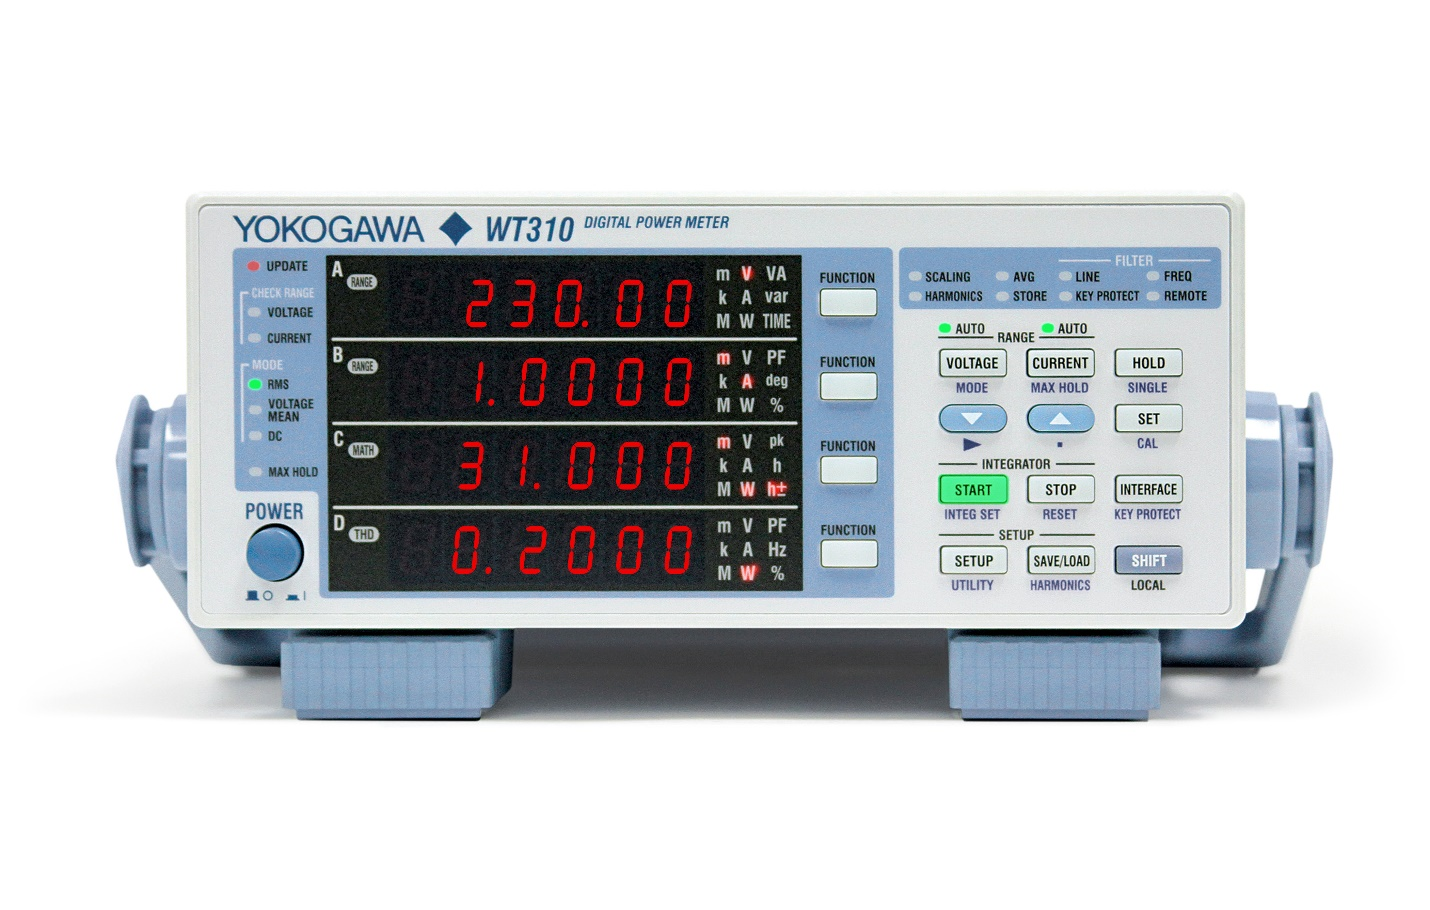
\includegraphics[width = 2.5in]{./Figures/MS/fig311.png}
		\rule{35em}{0.5pt}
	\caption{Digital Power Meter(Front)}
	\label{fig:Digital Power Meter(Front)} 
\end{figure}
\begin{figure}[htbp]
	\centering
		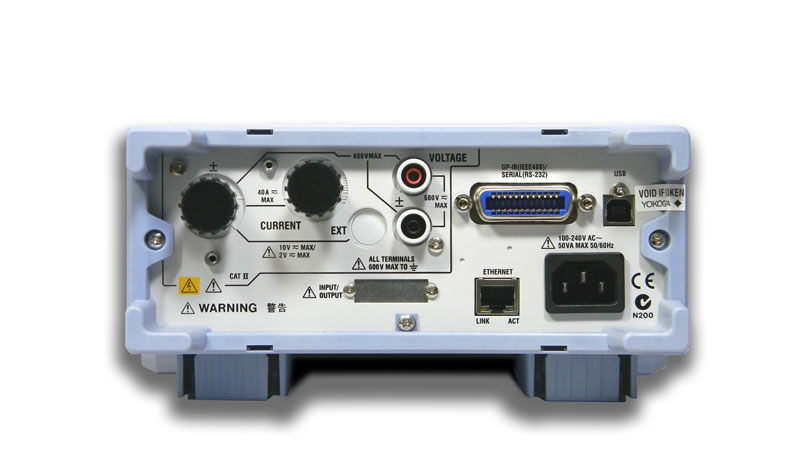
\includegraphics[width = 2.5in]{./Figures/MS/fig312.png}
		\rule{35em}{0.5pt}
	\caption{Digital Power Meter(Back)}
	\label{fig:Digital Power Meter(Back)} 
\end{figure}

\subsubsection{Measurement of electrical quantities in Simulink environment}
The selected motor model had a port for real and reactive power designated as (W) and (VAR):
\begin{figure}[htbp]
	\centering
		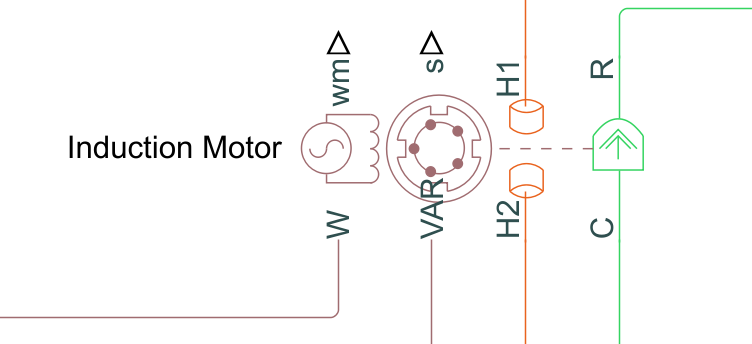
\includegraphics[width = 4.5in]{./Figures/MS/fig324.png}
		\rule{35em}{0.5pt}
	\caption{Induction Motor model in simulink}
	\label{fig:Induction Motor model in simulink} 
\end{figure}

As apparent from the symbol, this model doesn’t require a separate power source and has one embedded inside, as clear from the block settings as well:
\begin{figure}[htbp]
	\centering
		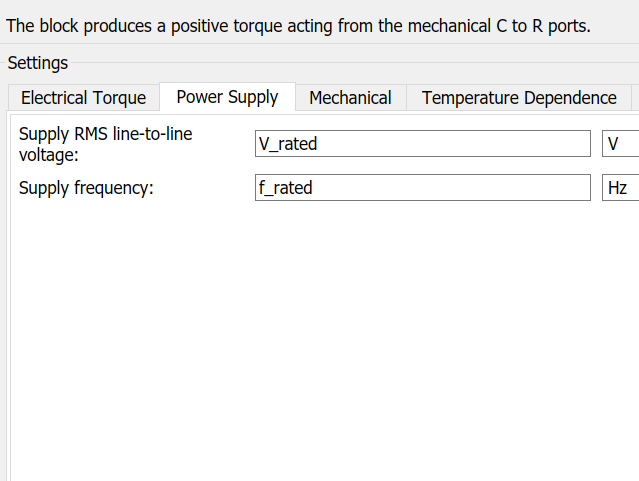
\includegraphics[width = 4.5in]{./Figures/MS/fig325.png}
		\rule{35em}{0.5pt}
	\caption{Induction Motor model properties in simulink}
	\label{fig:Induction Motor model properties in simulink} 
\end{figure}
The block assumes ideal power supply, so the frequency and voltage were assumed to be constant during all calculations. When implementing a real system, these may subject to changes, either due to loading conditions or instrument accuracies, which will affect the loss calculations, while the PID controller only requires the mechanical quantities, so the operation will remain unaffected by electrical measurements, only the calculated results. Current in an AC circuit can be given as:
\begin{equation}
	I_rms=\frac{S}{V_rms}
\end{equation}
Where S is the apparent power of the system. So, current was calculated as:
\begin{figure}[htbp]
	\centering
		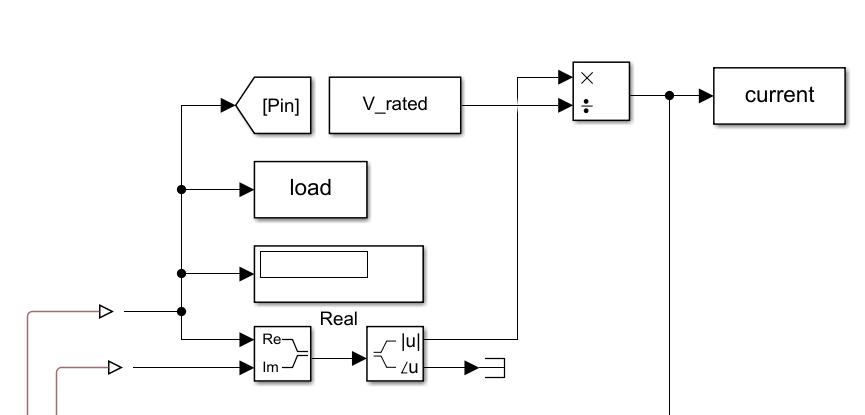
\includegraphics[width = 4.5in]{./Figures/MS/fig326.png}
		\rule{35em}{0.5pt}
	\caption{Current Measurement in Simulink}
	\label{fig:Current Measurement in Simulink} 
\end{figure}

\subsection{Mechanical Sensors}
\subsubsection{Torque}
\paragraph{Sensors in the market}
Torque sensors have two types:
\begin{itemize}
 \item Rotary Torque sensor
 \item Reaction Torque sensor
\end{itemize}
Rotary torque sensors are mounted on the motor shaft and provide the instantaneous torque, while reaction torque sensors are mounted on the body of the motor, and use newton’s 3rd law, i.e. measure the reaction of the torque produced on the motor body, so they lag a bit behind the instantaneous torque. The reaction torque sensors are suitable only for cases where the torque is stable and not changing rapidly.
\begin{figure}[htbp]
	\centering
		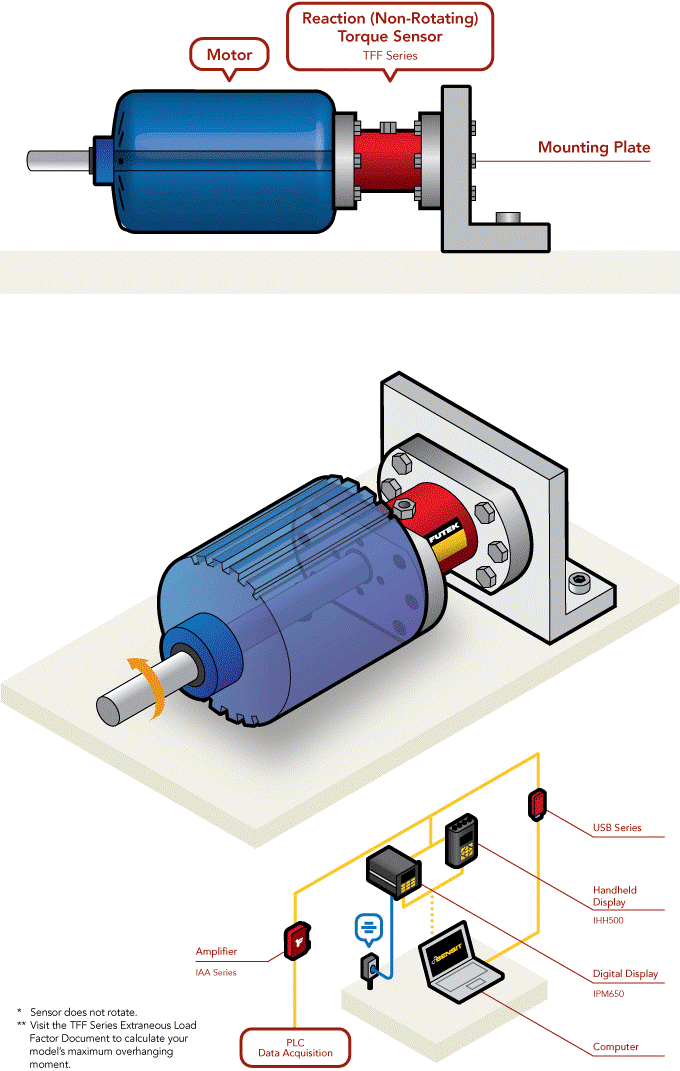
\includegraphics[width = 2.5in]{./Figures/MS/fig313.png}
		\rule{35em}{0.5pt}
	\caption{Reaction Torque Sensor}
	\label{fig:Reaction Torque Sensor} 
\end{figure}
\begin{figure}[htbp]
	\centering
		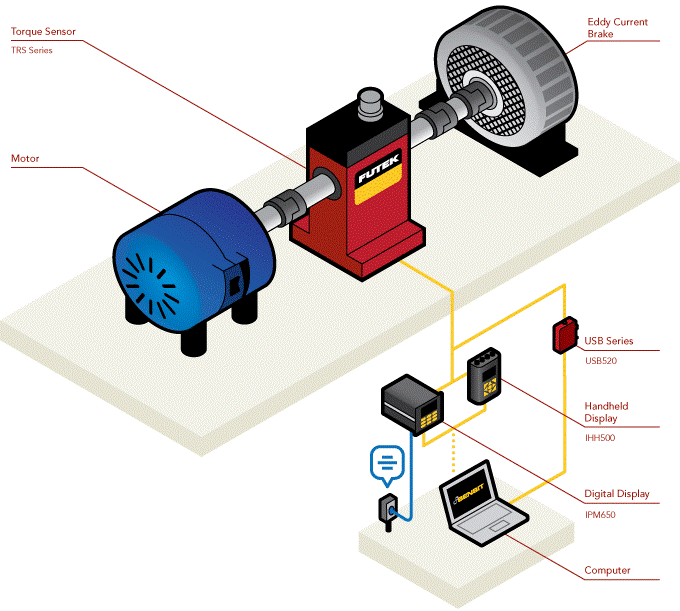
\includegraphics[width = 2.5in]{./Figures/MS/fig314.png}
		\rule{35em}{0.5pt}
	\caption{Rotary Torque Sensor}
	\label{fig:Rotary Torque Sensor} 
\end{figure}

\paragraph{Measurement of torque in Simulink environment}
\begin{figure}[htbp]
	\centering
		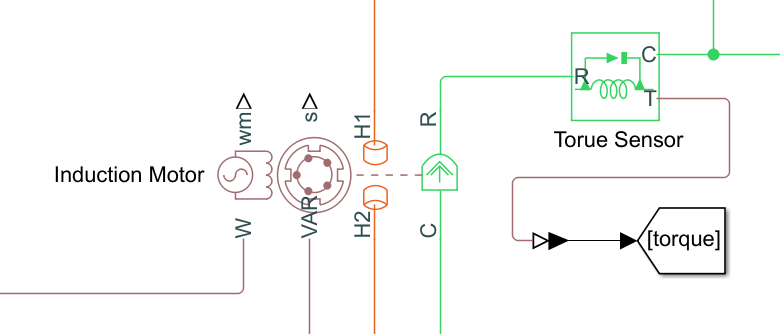
\includegraphics[width = 4.5in]{./Figures/MS/fig327.png}
		\rule{35em}{0.5pt}
	\caption{Torque Measurement in Simulink}
	\label{fig:Torque Measurement in Simulink} 
\end{figure}
The torque sensor in the Simulink environment is connected to the rotating end of the mechanical port of the motor, so it resembles the rotary torque sensor. But as defined by IEC standards, the motors will be tested in steady state, so the reaction torque sensors can also be used for this setup, when it is implemented practically.

\subsubsection{Angular Speed}
\paragraph{Sensors in the market}
Rotary torque sensors have an added benefit of finding the speed as well without requiring the installation of additional hardware, as they are already interacting directly with the shaft. Apart from that, angular speed sensors use different techniques, including on-shaft tachometers, optical sensors, etc. and indirect measurement of speed can also be done using acoustic analysis.
\begin{figure}[htbp]
	\centering
		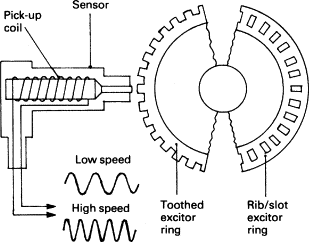
\includegraphics[width = 4.5in]{./Figures/MS/fig315.png}
		\rule{35em}{0.5pt}
	\caption{Optical Speed Sensor}
	\label{fig:Optical Speed Sensor} 
\end{figure}
\begin{figure}[htbp]
	\centering
		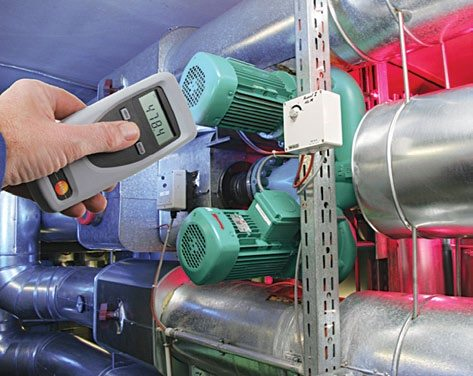
\includegraphics[width = 4.5in]{./Figures/MS/fig316.png}
		\rule{35em}{0.5pt}
	\caption{Speed Measurement using acoustics}
	\label{fig:Speed Measurement using acoustics} 
\end{figure}

\paragraph{Measurement of angular speed in Simulink environment}
\begin{figure}[htbp]
	\centering
		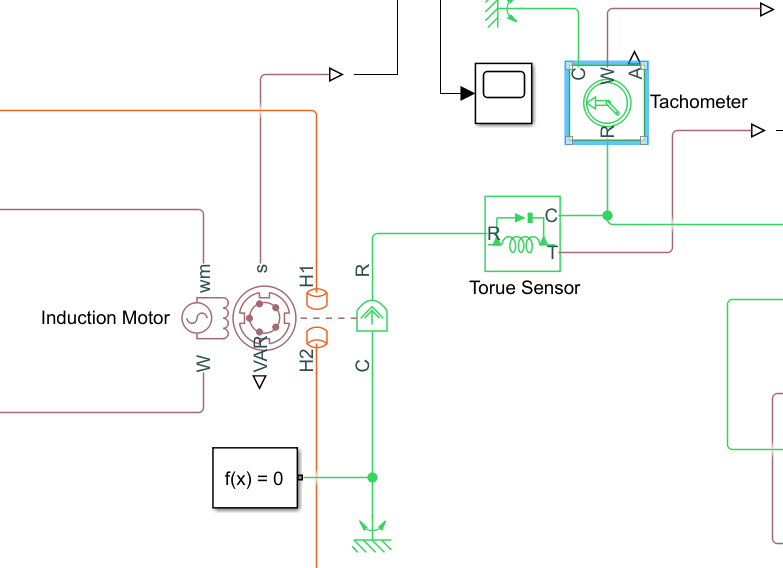
\includegraphics[width = 4.5in]{./Figures/MS/fig328.png}
		\rule{35em}{0.5pt}
	\caption{Speed Measurement in Simulink}
	\label{fig:Speed Measurement in Simulink} 
\end{figure}
Simulink provides a rotational motion sensor, that connects to the rotating port and provides angular position at the A port of the block and angular speed at the W port. The C port must be connected to mechanical zero reference. This resembles an on-shaft speed sensors, which are not commonly used or mostly available in motors with built-in rotary encoders, such as those to be used in robotics, etc.

\subsection{Thermal Sensors}
\subsubsection{Sensors in the market}
Three most commonly used sensors for temperature measurement are:
\begin{itemize}
	\item Thermistors
	\item Thermocouples
	\item RTD(Resistance Temperature Detectors)
\end{itemize}
A thermistor is a type of temperature dependent resistor. 
Thermistors are of two opposite fundamental types:
\begin{itemize}
	\item With NTC(negative temperature coefficient) thermistors, resistance decreases as temperature rises. 
	\item With PTC(positive temperature coefficient) thermistors, resistance increases as temperature rises. 
\end{itemize}
The thermistor is connected with another resistor in series, and the voltage of the thermistor is measured with an adc, which provides the temperature. Some calibration is required beforehand.
\begin{figure}[htbp]
	\centering
		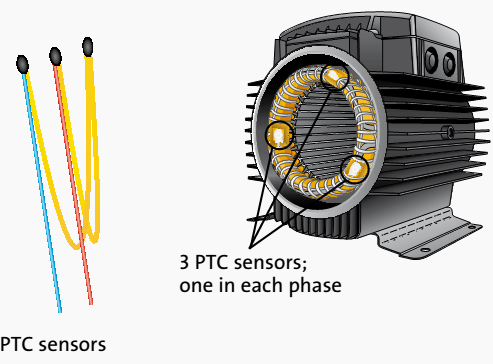
\includegraphics[width = 4.5in]{./Figures/MS/fig330.png}
		\rule{35em}{0.5pt}
	\caption{Thermistors installed on machine winding}
	\label{fig:Thermistors installed on machine winding} 
\end{figure}
A thermocouple consists of two different electrical conductors forming an electrical junction. A thermocouple produces a temperature-dependent voltage due thermoelectric effect, and this voltage can be used to measure temperature.
\begin{figure}[htbp]
	\centering
		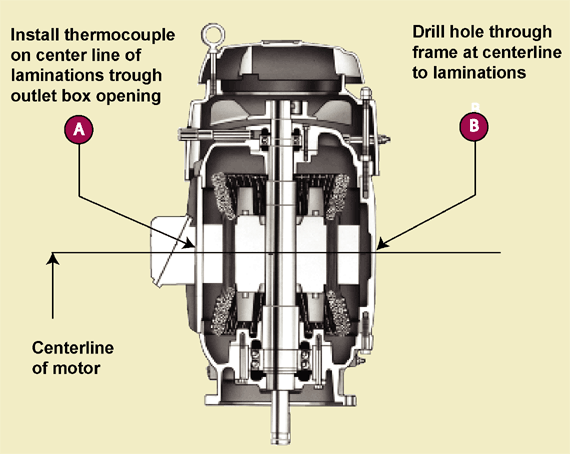
\includegraphics[width = 4.5in]{./Figures/MS/fig331.png}
		\rule{35em}{0.5pt}
	\caption{Installing a thermocouple on machine winding}
	\label{fig:Installing a thermocouple on machine winding} 
\end{figure}
An RTD consist of a fine wire wrapped around a ceramic or glass core The RTD wire is a pure material, typically platinum, nickel, or copper. The material has an accurate resistance/temperature relationship which is used to provide an indication of temperature.

RTDs have a range from -240 to 649\textdegree C, and thermocouples from zero to 1800\textdegree C and RTDs work better in below-freezing temps while thermocouples work better in very high temps. Thermistors have a very high accuracy in a range of about 50\textdegree C around the target temperature. 

\subsubsection{Measurement of electrical quantities in Simulink environment}
\begin{figure}[htbp]
	\centering
		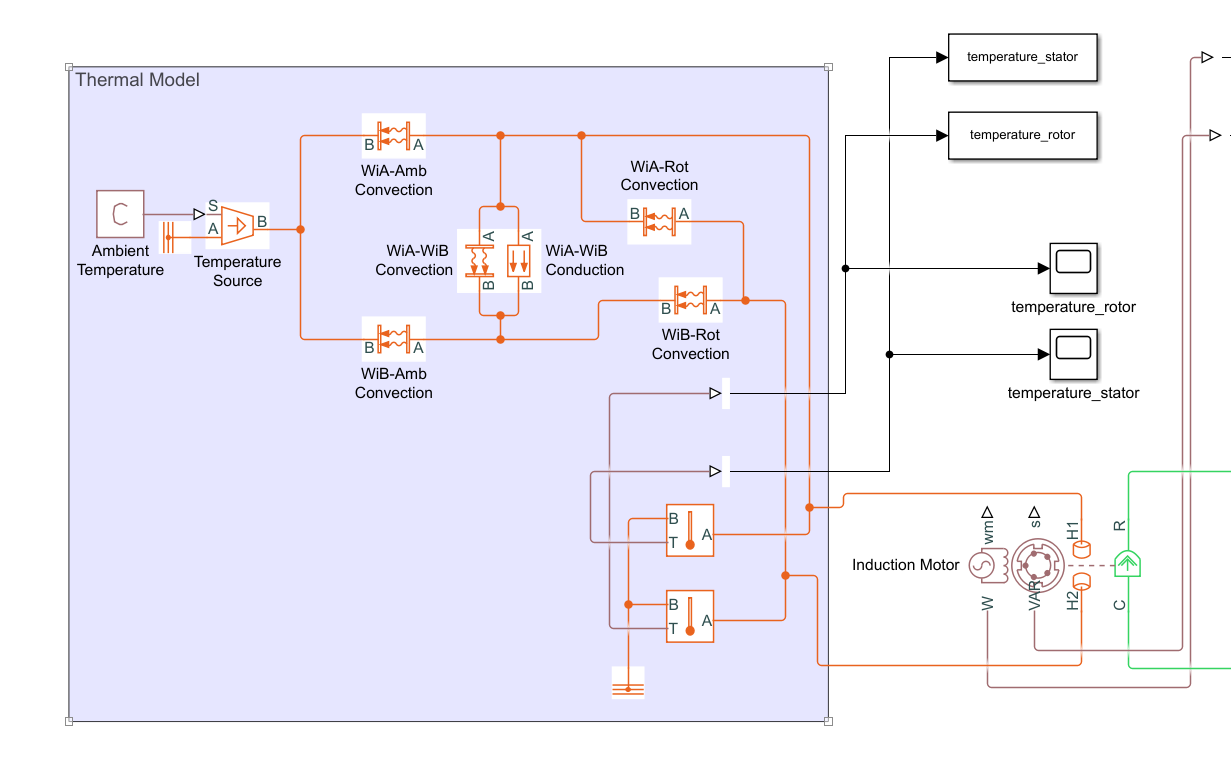
\includegraphics[width = 4.5in]{./Figures/MS/fig329.png}
		\rule{35em}{0.5pt}
	\caption{Temperature Measurement in Simulink}
	\label{fig:Temperature Measurement in Simulink} 
\end{figure}
In Simulink, the motor has two thermal ports, one for the stator, and the other for the rotor. The heat flow due to convection and conduction with ambiance, etc. has to be modeled using the respective blocks, after which thermal sensors are placed. Calculations in the IEC standard only require the winding temperature, so only the stator temperature is used, but the rotor model is also required for the thermal system to work properly. % Experimental Setup
% % Chapter 1
\setstretch{1.8}
\chapter{Algorithms and Flowcharts} % Write in your own chapter title
\label{Chapter4}
\lhead{Chapter 4. \emph{Algorithms and Flowcharts}} % Write in your own chapter title to set the page header

This chapter discusses the process as defined by the IEC standard, and the algorithms and their flowcharts developed to automate the process of motor testing. As described in earlier chapters, the systems were implemented in Simulink and the calling scripts were written in MATLAB.

\section{The Process as defined by IEC-60034-2-1}
Following figure is taken from IEC-60034-2-1:2014 which shows the tests to be performed for separating the losses of an induction motor, smaller than 2 MW.
\begin{figure}[htbp]
	\centering
		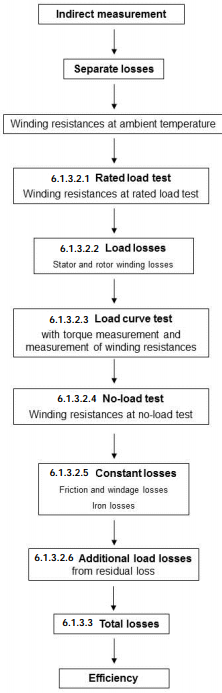
\includegraphics[width = 2.5in]{./Figures/MS/fig41.png}
		\rule{35em}{0.5pt}
	\caption{IEC 60034-2-1 method 2-1-1B, for induction motors}
	\label{fig:IEC 60034-2-1 method 2-1-1B, for induction motors} 
\end{figure}
\newpage

\section{Flowcharts}
\subsection{Rated load test}
The first test in the IEC standard method was the rated load test. In this test, the motor is loaded to its rated power, and is allowed to run till it reaches the thermal equilibrium, and the voltage, current, input power, speed, torque and temperature need to be measured.
Once the test is complete, the stator copper losses are calculated from the data using I\textsuperscript{2}R, and then a temperature correction is applied using temperature correction factor k. The process is illustrated by the following flowchart:
\begin{figure}[htbp]
	\centering
		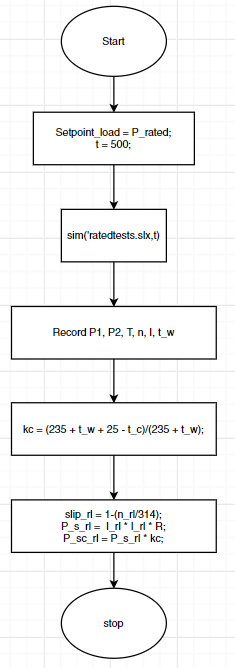
\includegraphics[width = 2.5in]{./Figures/MS/fig42.png}
		\rule{35em}{0.5pt}
	\caption{Rated load test flowchart}
	\label{fig:Rated load test flowchart} 
\end{figure}
\newpage

\subsection{Load Curve test}
The next test in the IEC standard method is the load curve test. In this test, the motor is loaded  to 6 different load points (125\%, 115\%, 100\%, 75\%, 50\%, 25\%), and is allowed to run till it reaches the thermal equilibrium, and the voltage, current, input power, speed, torque and temperature need to be measured.
Once the test is complete, the stator copper losses are calculated from the data using I\textsuperscript{2}R for each load point and then a temperature correction is applied using temperature correction factor k. The process is illustrated by the following flowchart:
\begin{figure}[htbp]
	\centering
		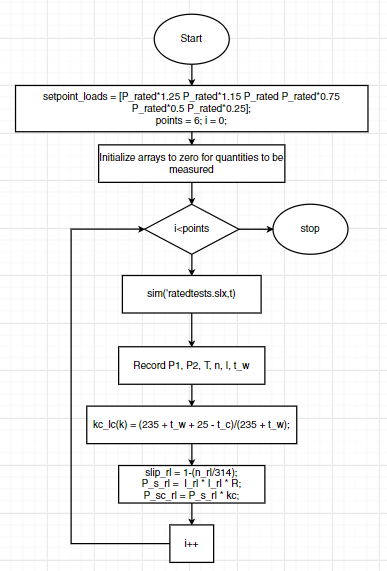
\includegraphics[width = 4.5in]{./Figures/MS/fig43.png}
		\rule{35em}{0.5pt}
	\caption{Load curve test flowchart}
	\label{fig:Load curve test flowchart} 
\end{figure}
\newpage

\subsection{No Load test}
The no-load test consists of two stages. In the first stage, the motor is allowed to run at its rated speed and the input power, voltage and current are measure. The output power is assumed zero in the case as there is no loading torque. In the next stage, the motor is disconnected from the source, and rotated to its rated speed using another motor, and the torque required to run the motor at its rated speed is measured. This torque, multiplied by the motor rated speed, provides us with the friction and windage losses. The iron losses are calculated by subtracting friction and windage losses and no load stator copper losses from the no load input power measured in the first stage. The process is illustrated by the following flowchart:
\begin{figure}[htbp]
	\centering
		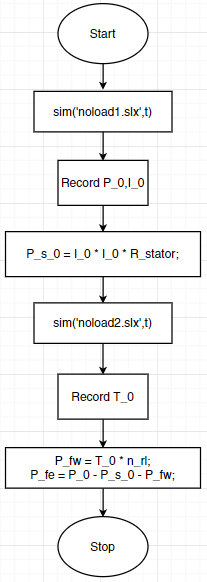
\includegraphics[width = 2.2in]{./Figures/MS/fig44.png}
		\rule{35em}{0.5pt}
	\caption{No load test flowchart}
	\label{fig:No load test flowchart} 
\end{figure}

\newpage
\subsection{Rotor loss and Additional losses}
The rotor copper losses are calculated for each load point by subtracting stator copper loss and iron loss from input power for each step and multiplying it by the slip. After this, the additional load losses can be calculated simply by subtracting all the losses from the input power for each load point. The process is illustrated by the following flowchart:
\begin{figure}[htbp]
	\centering
		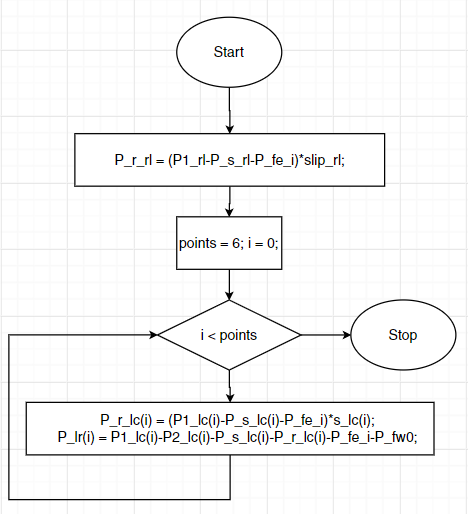
\includegraphics[width = 4.5in]{./Figures/MS/fig45.png}
		\rule{35em}{0.5pt}
	\caption{Rotor loss and PLL calculation flowchart}
	\label{fig:Rotor loss and PLL calculation flowchart} 
\end{figure}

\section{MATLAB scripts}
This section shows the scripts written in matlab to implement the above mentioned flowcharts.
\lstset{language=Matlab,%
    %basicstyle=\color{red},
    breaklines=true,%
    morekeywords={matlab2tikz},
    keywordstyle=\color{blue},%
    morekeywords=[2]{1}, keywordstyle=[2]{\color{black}},
    identifierstyle=\color{black},%
    stringstyle=\color{mylilas},
    commentstyle=\color{mygreen},%
    showstringspaces=false,%without this there will be a symbol in the places where there is a space
    numbers=left,%
    numberstyle={\tiny \color{black}},% size of the numbers
    numbersep=9pt, % this defines how far the numbers are from the text
    emph=[1]{for,end,break},emphstyle=[1]\color{red}, %some words to emphasise
    %emph=[2]{word1,word2}, emphstyle=[2]{style},    
}

\newpage
\section*{Rated load test script}
\lstinputlisting{ratedloadtest.m}

\section*{Load curve test script}
\lstinputlisting{loadcurvetest.m}

\section*{No load test script}
\lstinputlisting{noloadtest.m}

\section*{No load test script(alternate)}
\lstinputlisting{noloadtest.m}

\section*{Rotor loss and PLL calculation script}
\lstinputlisting{rotor_loss_later.m}
 % Experiment 1
% \setstretch{1.8}
\chapter{Results} % Write in your own chapter title
\label{Chapter5}
\lhead{Chapter 5. \emph{Results}} % Write in your own chapter title to set the page header

This chapter shows the results for the tests performed. The tests were performed on 1 hp and 1.5 hp motors, both rated for 220V and 50Hz.

\clearpage
\section{1 hp Motor}
\subsection{Motor characteristics}

\begin{figure}[hbtp!]
	\centering
		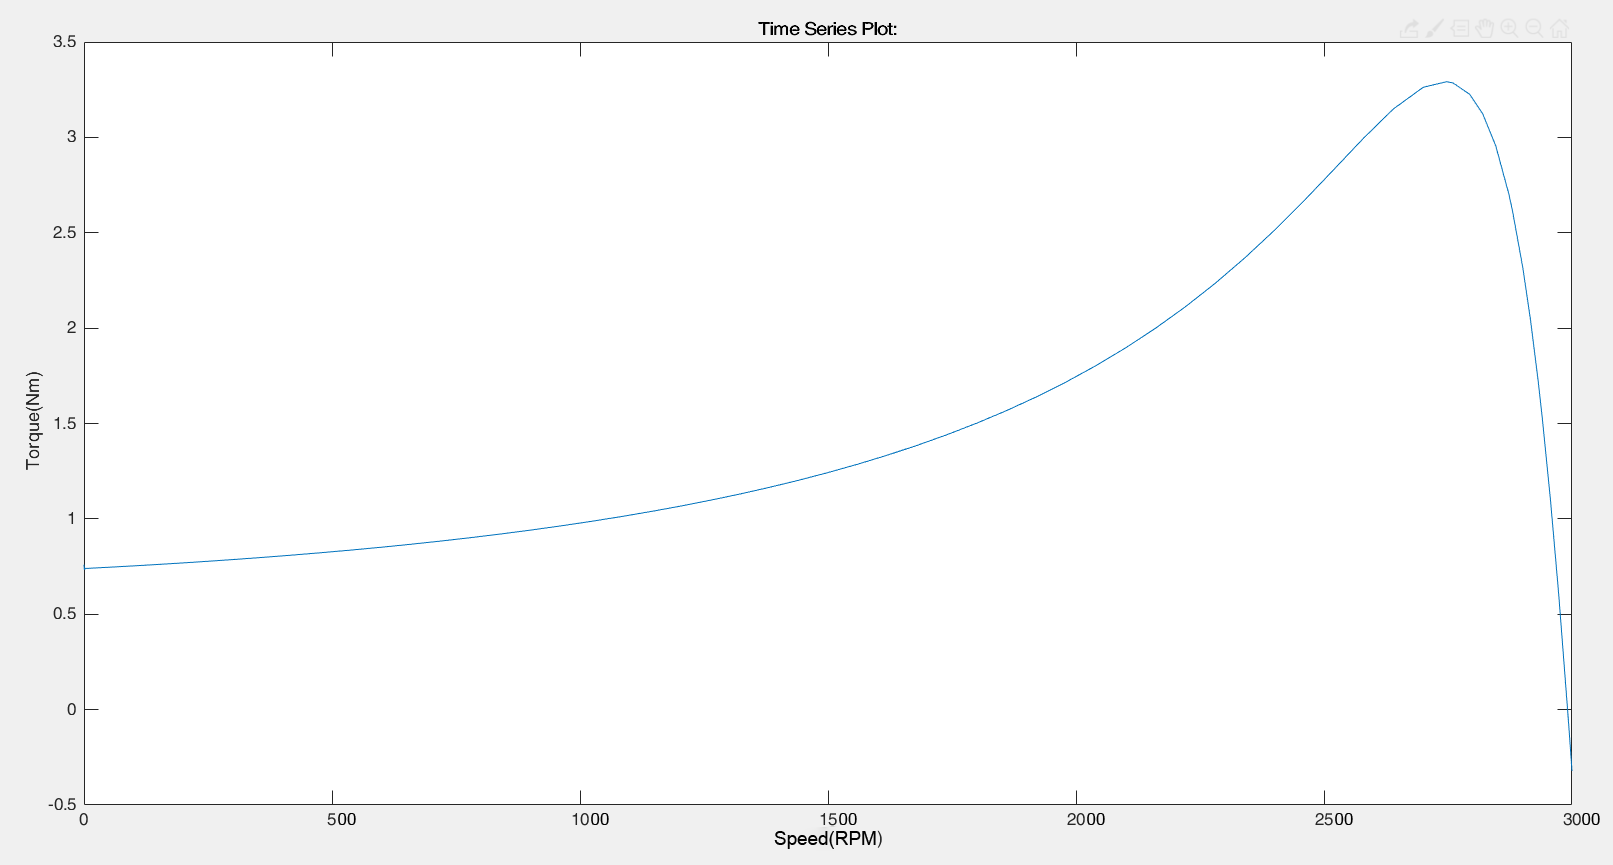
\includegraphics[width = 4.5in]{./Figures/MS/fig51.png}
		\rule{35em}{0.5pt}
	\caption{1hp motor torque-speed characteristics}
	\label{fig:1hp motor torque-speed characteristics} 
\end{figure}

\begin{figure}[hbtp!]
	\centering
		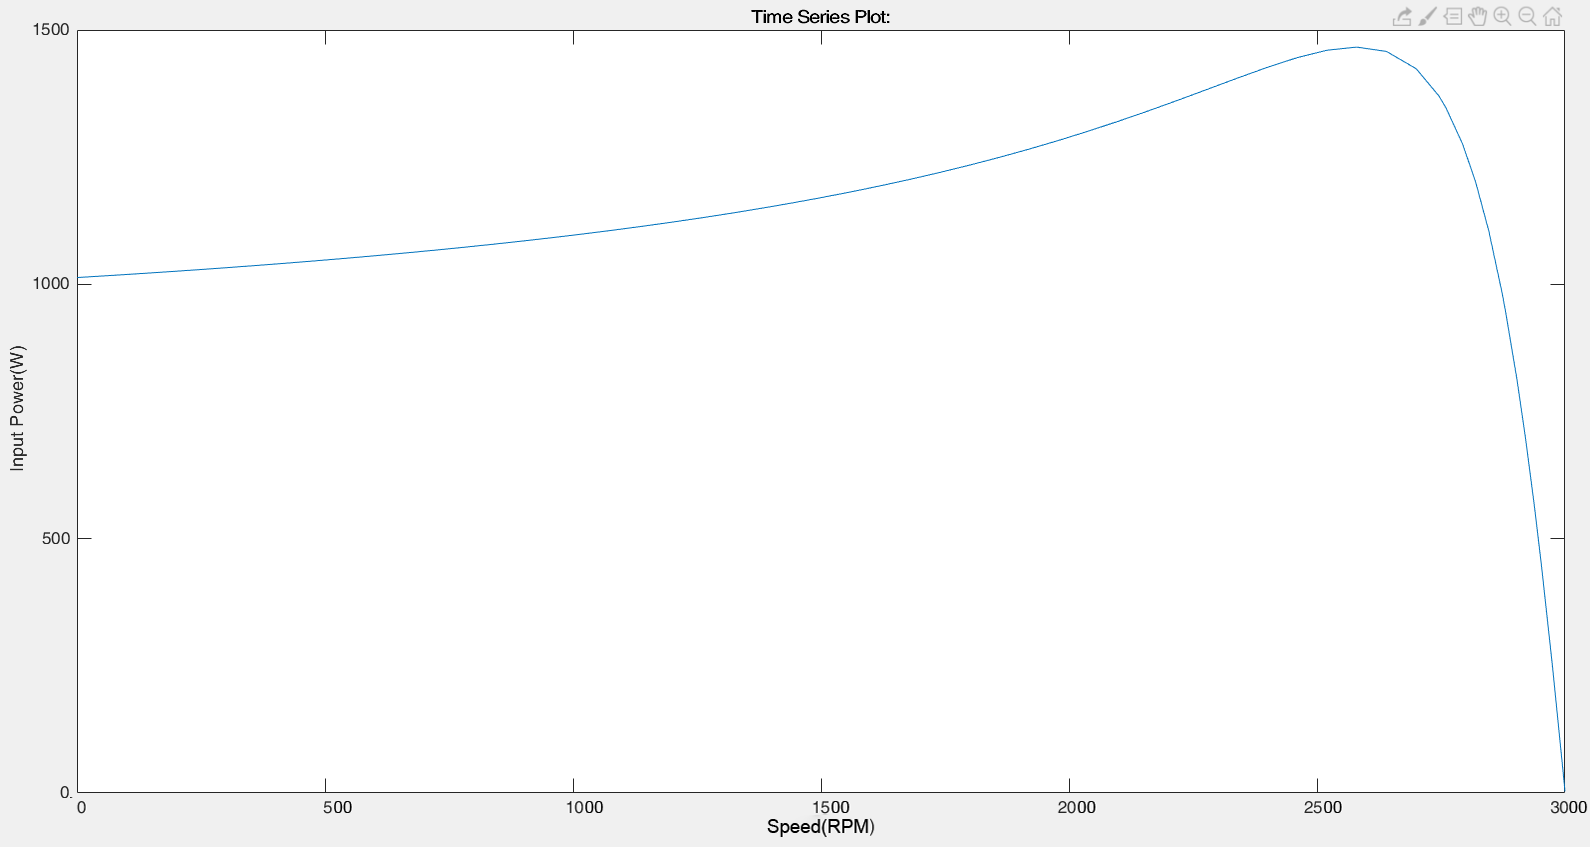
\includegraphics[width = 4.5in]{./Figures/MS/fig52.png}
		\rule{35em}{0.5pt}
	\caption{1hp motor input power characteristics}
	\label{fig:1hp motor input power characteristics} 
\end{figure}

\begin{figure}[hbtp!]
	\centering
		\includegraphics[width = 4.5in]{./Figures/MS/fig53.png}
		\rule{35em}{0.5pt}
	\caption{1hp motor output power characteristics}
	\label{fig:1hp motor output power characteristics} 
\end{figure}

\clearpage
\subsection{Method 1}
\subsubsection{Rated Load Test}
Following table shows the test results:
\begin{table}[hbtp!]
\begin{tabular}{>{\columncolor[HTML]{9B9B9B}}l llll}
    \cellcolor[HTML]{656565}{\color[HTML]{000000} Name} & \cellcolor[HTML]{656565}Symbol            & \cellcolor[HTML]{656565}Value     & \cellcolor[HTML]{656565}Unit &  \\
    {\color[HTML]{000000} Current}                      & I                                         & 4.7054                            & A                            &  \\
    {\color[HTML]{000000} Input   Power}                & \cellcolor[HTML]{F2F2F2}P1                & \cellcolor[HTML]{F2F2F2}978.26    & \cellcolor[HTML]{F2F2F2}W    &  \\
    {\color[HTML]{000000} Speed}                        & w                                         & 303.5737                          & rad/s                        &  \\
    {\color[HTML]{000000} Torque}                       & \cellcolor[HTML]{F2F2F2}T                 & \cellcolor[HTML]{F2F2F2}2.4574    & \cellcolor[HTML]{F2F2F2}Nm   &  \\
    {\color[HTML]{000000} stator resistance}            & R1                                        & 3.9                               & ohm                          &  \\
    {\color[HTML]{000000} slip}                         & \cellcolor[HTML]{F2F2F2}s                 & \cellcolor[HTML]{F2F2F2}0.0332    & \cellcolor[HTML]{F2F2F2}     &  \\
    {\color[HTML]{000000} Output   Power}               & P2                                        & 746.00201                         & W                            &  \\
    efficiency                                          & \cellcolor[HTML]{F2F2F2}P2/P1*100         & \cellcolor[HTML]{F2F2F2}76.25805  & \cellcolor[HTML]{F2F2F2}\%   &  \\
    Actual   losses                                     & P1-P2                                     & 232.25799                         & W                            &  \\
    Stator   Copper Loss                                & \cellcolor[HTML]{F2F2F2}Ps                & \cellcolor[HTML]{F2F2F2}86.34908  & \cellcolor[HTML]{F2F2F2}W    &  \\
    Rotor   Copper Loss                                 & Pr                                        & 26.68672                          & W                            &  \\
    Temp   correction factor                            & \cellcolor[HTML]{F2F2F2}k                 & \cellcolor[HTML]{F2F2F2}0.99631   & \cellcolor[HTML]{F2F2F2}     &  \\
    Temp corrected   slip                               & sc                                        & 0.03308                           &                              &  \\
    Temp   corrected Stator copper loss                 & \cellcolor[HTML]{F2F2F2}Ps,c              & \cellcolor[HTML]{F2F2F2}86.34908  & \cellcolor[HTML]{F2F2F2}W    &  \\
    Temp   corrected Rotor copper loss                  & Pr,c                                      & 26.58827                          & W                            &  \\
    Iron Loss                                           & \cellcolor[HTML]{F2F2F2}Pfe               & \cellcolor[HTML]{F2F2F2}88.20973  & \cellcolor[HTML]{F2F2F2}W    &  \\
    Friction\&Windage   Loss                            & Pfw                                       & 10.22740                          & W                            &  \\
    Calculated   Losses                                 & \cellcolor[HTML]{F2F2F2}Ps,c+Pr,c+Pfe+Pfw & \cellcolor[HTML]{F2F2F2}211.37448 & \cellcolor[HTML]{F2F2F2}W    &  \\
    Residual   Losses                                   & P\_Lr                                     & 20.88351                          & W                            & 
\end{tabular}
\end{table}

\subsubsection{Load curve test}
Following table shows the test results:
\begin{table}[hbtp!]
\begin{tabular}{lllllll}
    \rowcolor[HTML]{343434} 
    Load   points                                & 125\%    & 115\%    & 100\%    & 75\%     & 50\%     & 25\%     \\
    \rowcolor[HTML]{F2F2F2} 
    \cellcolor[HTML]{9B9B9B}Input   Power        & 1443.1   & 1171     & 978.26   & 722.1448 & 499.2    & 293.46   \\
    \cellcolor[HTML]{9B9B9B}Current              & 7.8101   & 5.8201   & 4.7054   & 3.3768   & 2.2977   & 1.3397   \\
    \rowcolor[HTML]{F2F2F2} 
    \cellcolor[HTML]{9B9B9B}Speed                & 289.0265 & 299.4447 & 303.5737 & 307.472  & 310.0261 & 311.9381 \\
    \cellcolor[HTML]{9B9B9B}Torque               & 3.2327   & 2.865    & 2.4574   & 1.8197   & 1.2031   & 0.5979   \\
    \rowcolor[HTML]{F2F2F2} 
    \cellcolor[HTML]{9B9B9B}slip                 & 0.0795   & 0.0464   & 0.0332   & 0.0208   & 0.0127   & 0.0066   \\
    \cellcolor[HTML]{9B9B9B}Output   Power       & 934.3360 & 857.9091 & 746.0020 & 559.5068 & 372.9924 & 186.5078 \\
    \rowcolor[HTML]{F2F2F2} 
    \cellcolor[HTML]{9B9B9B}Actual   Losses      & 508.7640 & 313.0909 & 232.2580 & 162.6380 & 126.2076 & 106.9522 \\
    \cellcolor[HTML]{9B9B9B}Efficiency           & 64.7451  & 73.2629  & 76.2581  & 77.4785  & 74.7180  & 63.5548  \\
    \rowcolor[HTML]{F2F2F2} 
    \cellcolor[HTML]{9B9B9B}Stator   Copper Loss & 237.8909 & 132.1069 & 86.3491  & 44.4708  & 20.5898  & 6.9997   \\
    \cellcolor[HTML]{9B9B9B}Rotor   Copper Loss  & 88.8388  & 44.0684  & 26.6867  & 12.2548  & 4.9408   & 1.3018   \\
    \rowcolor[HTML]{F2F2F2} 
    \cellcolor[HTML]{9B9B9B}Calculated   Losses  & 425.1668 & 274.6124 & 211.4729 & 155.1628 & 123.9677 & 106.7387 \\
    \cellcolor[HTML]{9B9B9B}P\_lr                & 83.5972  & 38.4785  & 20.7851  & 7.4752   & 2.2399   & 0.2136  
\end{tabular}
\end{table}

\subsubsection{No load test}
Following table shows the test results:
\begin{table}[hbtp!]
\begin{tabular}{llll}
    \rowcolor[HTML]{656565} 
    Name                                                              & Symbol  & Value    & Unit  \\
    \cellcolor[HTML]{656565}Voltage                                   & V\_0    & 220      & V     \\
    \rowcolor[HTML]{F2F2F2} 
    \cellcolor[HTML]{656565}Current                                   & I\_0    & 1.5107   & A     \\
    \cellcolor[HTML]{656565}Input   Power                             & P\_0    & 106.4249 & W     \\
    \rowcolor[HTML]{F2F2F2} 
    \cellcolor[HTML]{656565}Stator   Copper Loss                      & P\_s\_0 & 7.9877   & W     \\
    \cellcolor[HTML]{656565}Speed at   rated power                    & n\_rl   & 303.5737 & rad/s \\
    \rowcolor[HTML]{F2F2F2} 
    \cellcolor[HTML]{656565}Torque   Req. to rotate unenergized motor & T\_0    & 0.0307   & Nm    \\
    \cellcolor[HTML]{656565}Friction\&Windage   Loss                  & P\_fw   & 10.2274  & W     \\
    \rowcolor[HTML]{F2F2F2} 
    \cellcolor[HTML]{656565}Iron Loss                                 & P\_fe   & 88.2097  & W    
\end{tabular}
\end{table}

\begin{figure}[hbtp!]
	\centering
		\includegraphics[width = 4.5in]{./Figures/MS/fig54.png}
		\rule{35em}{0.5pt}
	\caption{Bar graph for losses at different load points for 1hp motor(method1)}
	\label{fig:Bar graph for losses at different load points for 1hp motor(method1)} 
\end{figure}

\begin{figure}[hbtp!]
	\centering
		\includegraphics[width = 4.5in]{./Figures/MS/fig55.png}
		\rule{35em}{0.5pt}
	\caption{Line chart for losses at different load points for 1hp motor(method1)}
	\label{fig:Line chart for losses at different load points for 1hp motor(method1)} 
\end{figure}

\begin{figure}[hbtp!]
	\centering
		\includegraphics[width = 4.5in]{./Figures/MS/fig56.png}
		\rule{35em}{0.5pt}
	\caption{Percentage load vs efficiency for 1hp motor(method1)}
	\label{fig:Percentage load vs efficiency for 1hp motor(method1)} 
\end{figure}

\begin{figure}[hbtp!]
	\centering
		\includegraphics[width = 4.5in]{./Figures/MS/fig57.png}
		\rule{35em}{0.5pt}
	\caption{Pie chart for loss distribution at rated load for 1hp motor(method1)}
	\label{fig:Pie chart for loss distribution at rated load for 1hp motor(method1)} 
\end{figure}

\clearpage
\subsection{Method 2}
\subsubsection{Rated Load Test}
Following table shows the test results:
\begin{table}[hbtp!]
\begin{tabular}{
    >{\columncolor[HTML]{9B9B9B}}l llll}
    \cellcolor[HTML]{656565}{\color[HTML]{000000} Name} & \cellcolor[HTML]{656565}Symbol            & \cellcolor[HTML]{656565}Value     & \cellcolor[HTML]{656565}Unit &  \\
    {\color[HTML]{000000} Current}                      & I                                         & 4.7048                            & A                            &  \\
    {\color[HTML]{000000} Input   Power}                & \cellcolor[HTML]{F2F2F2}P1                & \cellcolor[HTML]{F2F2F2}978.13    & \cellcolor[HTML]{F2F2F2}W    &  \\
    {\color[HTML]{000000} Speed}                        & w                                         & 303.6252                          & rad/s                        &  \\
    {\color[HTML]{000000} Torque}                       & \cellcolor[HTML]{F2F2F2}T                 & \cellcolor[HTML]{F2F2F2}2.4569    & \cellcolor[HTML]{F2F2F2}Nm   &  \\
    {\color[HTML]{000000} stator   resistance}          & R1                                        & 3.9                               & ohm                          &  \\
    {\color[HTML]{000000} slip}                         & \cellcolor[HTML]{F2F2F2}s                 & \cellcolor[HTML]{F2F2F2}0.0330    & \cellcolor[HTML]{F2F2F2}     &  \\
    {\color[HTML]{000000} Output   Power}               & P2                                        & 745.97675                         & W                            &  \\
    efficiency                                          & \cellcolor[HTML]{F2F2F2}P2/P1*100         & \cellcolor[HTML]{F2F2F2}76.26560  & \cellcolor[HTML]{F2F2F2}\%   &  \\
    Actual   losses                                     & P1-P2                                     & 232.15325                         & W                            &  \\
    Stator   Copper Loss                                & \cellcolor[HTML]{F2F2F2}Ps                & \cellcolor[HTML]{F2F2F2}86.32706  & \cellcolor[HTML]{F2F2F2}W    &  \\
    Rotor   Copper Loss                                 & Pr                                        & 26.55133                          & W                            &  \\
    Temp   correction factor                            & \cellcolor[HTML]{F2F2F2}k                 & \cellcolor[HTML]{F2F2F2}0.99631   & \cellcolor[HTML]{F2F2F2}     &  \\
    Temp corrected   slip                               & sc                                        & 0.03292                           &                              &  \\
    Temp   corrected Stator copper loss                 & \cellcolor[HTML]{F2F2F2}Ps,c              & \cellcolor[HTML]{F2F2F2}86.32706  & \cellcolor[HTML]{F2F2F2}W    &  \\
    Temp   corrected Rotor copper loss                  & Pr,c                                      & 26.45339                          & W                            &  \\
    Iron Loss                                           & \cellcolor[HTML]{F2F2F2}Pfe               & \cellcolor[HTML]{F2F2F2}88.20973  & \cellcolor[HTML]{F2F2F2}W    &  \\
    Friction\&Windage   Loss                            & Pfw                                       & 10.22740                          & W                            &  \\
    Calculated   Losses                                 & \cellcolor[HTML]{F2F2F2}Ps,c+Pr,c+Pfe+Pfw & \cellcolor[HTML]{F2F2F2}211.21757 & \cellcolor[HTML]{F2F2F2}W    &  \\
    Residual   Losses                                   & P\_Lr                                     & 20.93567                          & W                            & 
\end{tabular}
\end{table}

\subsubsection{Load curve test}
Following table shows the test results:
\begin{table}[hbtp!]
\begin{tabular}{lllllll}
    \rowcolor[HTML]{343434} 
    Load   points                                & 125\%    & 115\%    & 100\%    & 75\%     & 50\%     & 25\%     \\
    \rowcolor[HTML]{F2F2F2} 
    \cellcolor[HTML]{656565}Input   Power        & 1443.5   & 1171.1   & 978.13   & 722.1448 & 499.2    & 293.46   \\
    \cellcolor[HTML]{656565}Current              & 7.8095   & 5.8321   & 4.7048   & 3.3658   & 2.2795   & 1.3352   \\
    \rowcolor[HTML]{F2F2F2} 
    \cellcolor[HTML]{656565}Speed                & 289.0524 & 299.4647 & 303.6252 & 307.435  & 310.0315 & 311.9522 \\
    \cellcolor[HTML]{656565}Torque               & 3.233    & 2.862    & 2.4569   & 1.8191   & 1.2037   & 0.5976   \\
    \rowcolor[HTML]{F2F2F2} 
    \cellcolor[HTML]{656565}slip                 & 0.0795   & 0.0463   & 0.0330   & 0.0209   & 0.0126   & 0.0065   \\
    \cellcolor[HTML]{656565}Output   Power       & 934.5064 & 857.0680 & 745.9768 & 559.2550 & 373.1849 & 186.4226 \\
    \rowcolor[HTML]{F2F2F2} 
    \cellcolor[HTML]{656565}Actual   Losses      & 508.9936 & 314.0320 & 232.1532 & 162.8898 & 126.0151 & 107.0374 \\
    \cellcolor[HTML]{656565}Efficiency           & 64.7389  & 73.1849  & 76.2656  & 77.4436  & 74.7566  & 63.5257  \\
    \rowcolor[HTML]{F2F2F2} 
    \cellcolor[HTML]{656565}Stator   Copper Loss & 237.8543 & 132.6522 & 86.3271  & 44.1816  & 20.2649  & 6.9528   \\
    \cellcolor[HTML]{656565}Rotor   Copper Loss  & 88.7814  & 43.9872  & 26.5513  & 12.3304  & 4.9382   & 1.2932   \\
    \rowcolor[HTML]{F2F2F2} 
    \cellcolor[HTML]{656565}Calculated   Losses  & 425.0728 & 275.0766 & 211.3155 & 154.9491 & 123.6402 & 106.6831 \\
    \cellcolor[HTML]{656565}P\_lr                & 83.9208  & 38.9554  & 20.8377  & 7.9407   & 2.3749   & 0.3543   
\end{tabular}
\end{table}

\subsubsection{No load test}
Following table shows the test results:
\begin{table}[hbtp!]
\begin{tabular}{llll}
    \rowcolor[HTML]{656565} 
    Name                                                              & Symbol  & Value    & Unit  \\
    \cellcolor[HTML]{656565}Voltage                                 & V\_0    & 220      & V       \\
    \rowcolor[HTML]{F2F2F2} 
    \cellcolor[HTML]{656565}Current                                 & I\_0    & 1.5107   & A       \\
    \cellcolor[HTML]{656565}Input Power                             & P\_0    & 106.4249 & W       \\
    \rowcolor[HTML]{F2F2F2} 
    \cellcolor[HTML]{656565}Stator Copper Loss                      & P\_s\_0 & 7.9877   & W       \\
    \cellcolor[HTML]{656565}Speed at rated power                    & n\_rl   & 303.6252 & rad/s   \\
    \rowcolor[HTML]{F2F2F2} 
    \cellcolor[HTML]{656565}Torque Req. to rotate unenergized motor & T\_0    & 0.0307   & Nm      \\
    \cellcolor[HTML]{656565}Friction\&Windage Loss                  & P\_fw   & 10.2274  & W       \\
    \rowcolor[HTML]{F2F2F2} 
    \cellcolor[HTML]{656565}Iron Loss                               & P\_fe   & 88.2097  & W      
\end{tabular}
\end{table}

\begin{figure}[hbtp!]
	\centering
		\includegraphics[width = 4.5in]{./Figures/MS/fig58.png}
		\rule{35em}{0.5pt}
	\caption{Bar graph for losses at different load points for 1hp motor(method2)}
	\label{fig:Bar graph for losses at different load points for 1hp motor(method2)} 
\end{figure}

\begin{figure}[hbtp!]
	\centering
		\includegraphics[width = 4.5in]{./Figures/MS/fig59.png}
		\rule{35em}{0.5pt}
	\caption{Line chart for losses at different load points for 1hp motor(method2)}
	\label{fig:Line chart for losses at different load points for 1hp motor(method2)} 
\end{figure}

\begin{figure}[hbtp!]
	\centering
		\includegraphics[width = 4.5in]{./Figures/MS/fig510.png}
		\rule{35em}{0.5pt}
	\caption{Percentage load vs efficiency for 1hp motor(method2)}
	\label{fig:Percentage load vs efficiency for 1hp motor(method2)} 
\end{figure}

\begin{figure}[hbtp!]
	\centering
		\includegraphics[width = 4.5in]{./Figures/MS/fig511.png}
		\rule{35em}{0.5pt}
	\caption{Pie chart for loss distribution at rated load for 1hp motor(method2)}
	\label{fig:Pie chart for loss distribution at rated load for 1hp motor(method2)} 
\end{figure}

\clearpage
\section{1.5 hp Motor}
\subsection{Motor characteristics}

\begin{figure}[hbtp!]
	\centering
		\includegraphics[width = 4.5in]{./Figures/MS/fig512.png}
		\rule{35em}{0.5pt}
	\caption{1.5 hp motor torque-speed characteristics}
	\label{fig:1.5 hp motor torque-speed characteristics} 
\end{figure}

\begin{figure}[hbtp!]
	\centering
		\includegraphics[width = 4.5in]{./Figures/MS/fig513.png}
		\rule{35em}{0.5pt}
	\caption{1.5 hp motor input power characteristics}
	\label{fig:1.5 hp motor input power characteristics} 
\end{figure}

\begin{figure}[hbtp!]
	\centering
		\includegraphics[width = 4.5in]{./Figures/MS/fig514.png}
		\rule{35em}{0.5pt}
	\caption{1.5 hp motor output power characteristics}
	\label{fig:1.5 hp motor output power characteristics} 
\end{figure}

\clearpage
\subsection{Method 1}
\subsubsection{Rated Load Test}
Following table shows the test results:
\begin{table}[hbtp!]
\begin{tabular}{
    >{\columncolor[HTML]{9B9B9B}}l llll}
    \cellcolor[HTML]{656565}{\color[HTML]{000000} Name} & \cellcolor[HTML]{656565}Symbol            & \cellcolor[HTML]{656565}Value     & \cellcolor[HTML]{656565}Unit &  \\
    {\color[HTML]{000000} Current}                      & I                                         & 7.0225                            & A                            &  \\
    {\color[HTML]{000000} Input   Power}                & \cellcolor[HTML]{F2F2F2}P1                & \cellcolor[HTML]{F2F2F2}1473.5    & \cellcolor[HTML]{F2F2F2}W    &  \\
    {\color[HTML]{000000} Speed}                        & w                                         & 309.8536                          & rad/s                        &  \\
    {\color[HTML]{000000} Torque}                       & \cellcolor[HTML]{F2F2F2}T                 & \cellcolor[HTML]{F2F2F2}3.6114    & \cellcolor[HTML]{F2F2F2}Nm   &  \\
    {\color[HTML]{000000} stator   resistance}          & R1                                        & 3.5                               & ohm                          &  \\
    {\color[HTML]{000000} slip}                         & \cellcolor[HTML]{F2F2F2}s                 & \cellcolor[HTML]{F2F2F2}0.0132    & \cellcolor[HTML]{F2F2F2}     &  \\
    {\color[HTML]{000000} Output   Power}               & P2                                        & 1119.00529                        & W                            &  \\
    efficiency                                          & \cellcolor[HTML]{F2F2F2}P2/P1*100         & \cellcolor[HTML]{F2F2F2}75.94199  & \cellcolor[HTML]{F2F2F2}\%   &  \\
    Actual   losses                                     & P1-P2                                     & 354.49471                         & W                            &  \\
    Stator   Copper Loss                                & \cellcolor[HTML]{F2F2F2}Ps                & \cellcolor[HTML]{F2F2F2}172.60427 & \cellcolor[HTML]{F2F2F2}W    &  \\
    Rotor   Copper Loss                                 & Pr                                        & 15.72472                          & W                            &  \\
    Temp   correction factor                            & \cellcolor[HTML]{F2F2F2}k                 & \cellcolor[HTML]{F2F2F2}0.99631   & \cellcolor[HTML]{F2F2F2}     &  \\
    Temp   corrected slip                               & sc                                        & 0.01316                           &                              &  \\
    Temp   corrected Stator copper loss                 & \cellcolor[HTML]{F2F2F2}Ps,c              & \cellcolor[HTML]{F2F2F2}172.60427 & \cellcolor[HTML]{F2F2F2}W    &  \\
    Temp   corrected Rotor copper loss                  & Pr,c                                      & 15.66671                          & W                            &  \\
    Iron Loss                                           & \cellcolor[HTML]{F2F2F2}Pfe               & \cellcolor[HTML]{F2F2F2}95.08894 & \cellcolor[HTML]{F2F2F2}W    &  \\
    Friction\&Windage   Loss                            & Pfw                                       & 29.68700                          & W                            &  \\
    Calculated   Losses                                 & \cellcolor[HTML]{F2F2F2}Ps,c+Pr,c+Pfe+Pfw & \cellcolor[HTML]{F2F2F2}328.04692 & \cellcolor[HTML]{F2F2F2}W    &  \\
    Residual   Losses                                   & P\_Lr                                     & 20.93567                          & W                            & 
\end{tabular}
\end{table}

\subsubsection{Load curve test}
Following table shows the test results:
\begin{table}[hbtp!]
\begin{tabular}{
    >{\columncolor[HTML]{9B9B9B}}l llllll}
    \cellcolor[HTML]{656565}Load points & \cellcolor[HTML]{656565}125\% & \cellcolor[HTML]{656565}115\% & \cellcolor[HTML]{656565}100\% & \cellcolor[HTML]{656565}75\% & \cellcolor[HTML]{656565}50\% & \cellcolor[HTML]{656565}25\% \\
    Input Power                         & 2052.3                        & 1767.2                        & 1473.5                        & 1087.17                      & 741.54                       & 429.76                       \\
    Current                             & 9.4334                        & 7.9319                        & 7.0225                        & 5.7065                       & 3.7449                       & 2.4687                       \\
    Speed                               & 301.6                         & 305.2435                      & 309.8536                      & 312.4331                     & 313.1374                     & 313.6703                     \\
    Torque                              & 4.637697281                   & 4.215844072                   & 3.6114                        & 2.6862                       & 1.7868                       & 0.8919                       \\
    slip                                & 0.0395                        & 0.0279                        & 0.0132                        & 0.0050                       & 0.0027                       & 0.0011                       \\
    Output Power                        & 1398.7295                     & 1286.8590                     & 1119.0053                     & 839.2578                     & 559.5139                     & 279.7625                     \\
    Actual Losses                       & 653.5705                      & 480.3410                      & 354.4947                      & 247.9122                     & 182.0261                     & 149.9975                     \\
    Efficiency                          & 68.1542                       & 72.8191                       & 75.9420                       & 77.1966                      & 75.4530                      & 65.0974                      \\
    Stator Copper Loss                  & 311.4616                      & 220.2026                      & 172.6043                      & 113.9745                     & 49.0850                      & 21.3307                      \\
    Rotor Copper Loss                   & 64.9914                       & 40.4893                       & 15.9228                       & 4.3819                       & 1.6410                       & 0.3290                       \\
    Calculated Losses                   & 501.2289                      & 385.4679                      & 313.3030                      & 243.1323                     & 175.5020                     & 146.4356                     \\
    P\_lr                               & 152.3416                      & 94.8731                       & 41.1917                       & 4.7799                       & 6.5241                       & 3.5618                      
\end{tabular}
\end{table}

\subsubsection{No load test}
Following table shows the test results:
\begin{table}[hbtp!]
\begin{tabular}{llll}
    \rowcolor[HTML]{656565} 
    Name                                                              & Symbol  & Value    & Unit  \\
    \cellcolor[HTML]{9B9B9B}Voltage                                   & V\_0    & 220      & V     \\
    \rowcolor[HTML]{F2F2F2} 
    \cellcolor[HTML]{9B9B9B}Current                                   & I\_0    & 2.3112   & A     \\
    \cellcolor[HTML]{9B9B9B}Input   Power                             & P\_0    & 158.4717 & W     \\
    \rowcolor[HTML]{F2F2F2} 
    \cellcolor[HTML]{9B9B9B}Stator   Copper Loss                      & P\_s\_0 & 18.6958  & W     \\
    \cellcolor[HTML]{9B9B9B}Speed at   rated power                    & n\_rl   & 309.8536 & rad/s \\
    \rowcolor[HTML]{F2F2F2} 
    \cellcolor[HTML]{9B9B9B}Torque   Req. to rotate unenergized motor & T\_0    & 0.1858   & Nm    \\
    \cellcolor[HTML]{9B9B9B}Friction\&Windage   Loss                  & P\_fw   & 29.6870  & W     \\
    \rowcolor[HTML]{F2F2F2} 
    \cellcolor[HTML]{9B9B9B}Iron Loss                                 & P\_fe   & 95.0889 & W    
\end{tabular}
\end{table}

\begin{figure}[hbtp!]
	\centering
		\includegraphics[width = 4.5in]{./Figures/MS/fig515.png}
		\rule{35em}{0.5pt}
	\caption{Bar graph for losses at different load points for 1.5 hp motor(method1)}
	\label{fig:Bar graph for losses at different load points for 1.5 hp motor(method1)} 
\end{figure}

\begin{figure}[hbtp!]
	\centering
		\includegraphics[width = 4.5in]{./Figures/MS/fig516.png}
		\rule{35em}{0.5pt}
	\caption{Line chart for losses at different load points for 1.5 hp motor(method1)}
	\label{fig:Line chart for losses at different load points for 1.5 hp motor(method1)} 
\end{figure}

\begin{figure}[hbtp!]
	\centering
		\includegraphics[width = 4.5in]{./Figures/MS/fig517.png}
		\rule{35em}{0.5pt}
	\caption{Percentage load vs efficiency for 1.5 hp motor(method1)}
	\label{fig:Percentage load vs efficiency for 1.5 hp motor(method1)} 
\end{figure}

\begin{figure}[hbtp!]
	\centering
		\includegraphics[width = 4.5in]{./Figures/MS/fig518.png}
		\rule{35em}{0.5pt}
	\caption{Pie chart for loss distribution at rated load for 1.5 hp motor(method1)}
	\label{fig:Pie chart for loss distribution at rated load for 1.5 hp motor(method1)} 
\end{figure}

\clearpage
\subsection{Method 2}
\subsubsection{Rated Load Test}
Following table shows the test results:
\begin{table}[hbtp!]
\begin{tabular}{
    >{\columncolor[HTML]{9B9B9B}}l llll}
    \cellcolor[HTML]{656565}{\color[HTML]{000000} Name} & \cellcolor[HTML]{656565}Symbol            & \cellcolor[HTML]{656565}Value     & \cellcolor[HTML]{656565}Unit &  \\
    {\color[HTML]{000000} Current}                      & I                                         & 4.7048                            & A                            &  \\
    {\color[HTML]{000000} Input   Power}                & \cellcolor[HTML]{F2F2F2}P1                & \cellcolor[HTML]{F2F2F2}978.13    & \cellcolor[HTML]{F2F2F2}W    &  \\
    {\color[HTML]{000000} Speed}                        & w                                         & 303.6252                          & rad/s                        &  \\
    {\color[HTML]{000000} Torque}                       & \cellcolor[HTML]{F2F2F2}T                 & \cellcolor[HTML]{F2F2F2}2.4569    & \cellcolor[HTML]{F2F2F2}Nm   &  \\
    {\color[HTML]{000000} stator   resistance}          & R1                                        & 3.9                               & ohm                          &  \\
    {\color[HTML]{000000} slip}                         & \cellcolor[HTML]{F2F2F2}s                 & \cellcolor[HTML]{F2F2F2}0.0330    & \cellcolor[HTML]{F2F2F2}     &  \\
    {\color[HTML]{000000} Output   Power}               & P2                                        & 745.97675                         & W                            &  \\
    efficiency                                          & \cellcolor[HTML]{F2F2F2}P2/P1*100         & \cellcolor[HTML]{F2F2F2}76.26560  & \cellcolor[HTML]{F2F2F2}\%   &  \\
    Actual   losses                                     & P1-P2                                     & 232.15325                         & W                            &  \\
    Stator   Copper Loss                                & \cellcolor[HTML]{F2F2F2}Ps                & \cellcolor[HTML]{F2F2F2}86.32706  & \cellcolor[HTML]{F2F2F2}W    &  \\
    Rotor   Copper Loss                                 & Pr                                        & 26.55133                          & W                            &  \\
    Temp   correction factor                            & \cellcolor[HTML]{F2F2F2}k                 & \cellcolor[HTML]{F2F2F2}0.99631   & \cellcolor[HTML]{F2F2F2}     &  \\
    Temp corrected   slip                               & sc                                        & 0.03292                           &                              &  \\
    Temp   corrected Stator copper loss                 & \cellcolor[HTML]{F2F2F2}Ps,c              & \cellcolor[HTML]{F2F2F2}86.32706  & \cellcolor[HTML]{F2F2F2}W    &  \\
    Temp   corrected Rotor copper loss                  & Pr,c                                      & 26.45339                          & W                            &  \\
    Iron Loss                                           & \cellcolor[HTML]{F2F2F2}Pfe               & \cellcolor[HTML]{F2F2F2}88.20973  & \cellcolor[HTML]{F2F2F2}W    &  \\
    Friction\&Windage   Loss                            & Pfw                                       & 10.22740                          & W                            &  \\
    Calculated   Losses                                 & \cellcolor[HTML]{F2F2F2}Ps,c+Pr,c+Pfe+Pfw & \cellcolor[HTML]{F2F2F2}211.21757 & \cellcolor[HTML]{F2F2F2}W    &  \\
    Residual   Losses                                   & P\_Lr                                     & 20.93567                          & W                            & 
\end{tabular}
\end{table}

\subsubsection{Load curve test}
Following table shows the test results:
\begin{table}[hbtp!]
\begin{tabular}{
    >{\columncolor[HTML]{9B9B9B}}l llllll}
    \cellcolor[HTML]{656565}Load points & \cellcolor[HTML]{656565}125\% & \cellcolor[HTML]{656565}115\% & \cellcolor[HTML]{656565}100\% & \cellcolor[HTML]{656565}75\% & \cellcolor[HTML]{656565}50\% & \cellcolor[HTML]{656565}25\% \\
    Input Power                         & 2051.5                        & 1766.5                        & 1472.4                        & 1086.52                      & 740.89                       & 430.66                       \\
    Current                             & 9.4328                        & 7.9311                        & 7.0218                        & 5.7034                       & 3.7456                       & 2.4664                       \\
    Speed                               & 301.8                         & 305.2142                      & 309.8572                      & 312.4219                     & 313.1297                     & 313.6544                     \\
    Torque                              & 4.634621272                   & 4.216291378                   & 3.6111                        & 2.686156124                  & 1.78686                      & 0.889113                     \\
    slip                                & 0.0389                        & 0.0280                        & 0.0132                        & 0.0050                       & 0.0028                       & 0.0011                       \\
    Output Power                        & 1398.7287                     & 1286.8720                     & 1118.9253                     & 839.2140                     & 559.5189                     & 278.8743                     \\
    Actual Losses                       & 652.7713                      & 479.6280                      & 353.4747                      & 247.3060                     & 181.3711                     & 151.7857                     \\
    Efficiency                          & 68.1808                       & 72.8487                       & 75.9933                       & 77.2387                      & 75.5198                      & 64.7551                      \\
    Stator Copper Loss                  & 311.4220                      & 220.1582                      & 172.5699                      & 113.8507                     & 49.1033                      & 21.2910                      \\
    Rotor Copper Loss                   & 63.9136                       & 40.6064                       & 15.8949                       & 4.4105                       & 1.6538                       & 0.3459                       \\
    Calculated Losses                   & 500.1115                      & 385.5406                      & 313.2407                      & 243.0372                     & 175.5331                     & 146.4128                     \\
    P\_lr                               & 152.6598                      & 94.0874                       & 40.2340                       & 4.2688                       & 5.8380                       & 5.3729                      
\end{tabular}
\end{table}

\subsubsection{No load test}
\begin{table}[hbtp!]
\begin{tabular}{llll}
    \rowcolor[HTML]{656565} 
    Name                                                              & Symbol  & Value    & Unit  \\
    \cellcolor[HTML]{656565}Voltage                                 & V\_0    & 220      & V       \\
    \rowcolor[HTML]{F2F2F2} 
    \cellcolor[HTML]{656565}Current                                 & I\_0    & 1.5107   & A       \\
    \cellcolor[HTML]{656565}Input Power                             & P\_0    & 106.4249 & W       \\
    \rowcolor[HTML]{F2F2F2} 
    \cellcolor[HTML]{656565}Stator Copper Loss                      & P\_s\_0 & 7.9877   & W       \\
    \cellcolor[HTML]{656565}Speed at rated power                    & n\_rl   & 303.6252 & rad/s   \\
    \rowcolor[HTML]{F2F2F2} 
    \cellcolor[HTML]{656565}Torque Req. to rotate unenergized motor & T\_0    & 0.0307   & Nm      \\
    \cellcolor[HTML]{656565}Friction\&Windage Loss                  & P\_fw   & 10.2274  & W       \\
    \rowcolor[HTML]{F2F2F2} 
    \cellcolor[HTML]{656565}Iron Loss                               & P\_fe   & 88.2097  & W      
\end{tabular}
\end{table}

\begin{figure}[hbtp!]
	\centering
		\includegraphics[width = 4.5in]{./Figures/MS/fig519.png}
		\rule{35em}{0.5pt}
	\caption{Bar graph for losses at different load points for 1.5 hp motor(method2)}
	\label{fig:Bar graph for losses at different load points for 1.5 hp motor(method2)} 
\end{figure}

\begin{figure}[hbtp!]
	\centering
		\includegraphics[width = 4.5in]{./Figures/MS/fig520.png}
		\rule{35em}{0.5pt}
	\caption{Line chart for losses at different load points for 1.5 hp motor(method2)}
	\label{fig:Line chart for losses at different load points for 1.5 hp motor(method2)} 
\end{figure}

\begin{figure}[hbtp!]
	\centering
		\includegraphics[width = 4.5in]{./Figures/MS/fig521.png}
		\rule{35em}{0.5pt}
	\caption{Percentage load vs efficiency for 1.5 hp motor(method2)}
	\label{fig:Percentage load vs efficiency for 1.5 hp motor(method2)} 
\end{figure}

\begin{figure}[hbtp!]
	\centering
		\includegraphics[width = 4.5in]{./Figures/MS/fig522.png}
		\rule{35em}{0.5pt}
	\caption{Pie chart for loss distribution at rated load for 1.5 hp motor(method2)}
	\label{fig:Pie chart for loss distribution at rated load for 1.5 hp motor(method2)} 
\end{figure}

\clearpage
\section{Concluding Remarks}
\begin{itemize}
    \item The algorithms applied and results of the simulation serve as a preliminary analysis for the formation of the actual hardware test benches. 
    \item By replacing the dynamometer with a pump and connecting pressure transducers and flow rate sensors, this setup can be extended to a testbench for pump testing according to ISO-9906
    \item Since the algorithm has shown to be working on multiple setups, hence it can be used to test other setups as well, if they will be able to work or not before building the actual setup. Once such setup tested was using a dc supply will a single-phase motor to apply the phenomenon of dc injection braking, which was not successful.
\end{itemize}

 % Experiment 2

\bibliographystyle{ieeetr}
\bibliography{references}
%\input{./Chapters/Chapter6} % Results and Discussion

%\input{./Chapters/Chapter7} % Conclusion

%% ----------------------------------------------------------------
% Now begin the Appendices, including them as separate files

\addtocontents{toc}{\vspace{2em}} % Add a gap in the Contents, for aesthetics

\appendix % Cue to tell LaTeX that the following 'chapters' are Appendices

%% Appendix A

\chapter{I2C Bus Transactions}
\label{AppendixA}
\lhead{Appendix A. \emph{I2C Transactions}}





\section{Basics of I2C}
The I2C is a is a synchronous serial communication protocol that uses 2 wires, SCL (serial clock) and SDA (serial data), hence also called the “2-wire” interface. It transfers data in bytes, where the LSB of the starting bit indicates a read or write operation, so I2C devices mostly have a 7-bit address. The address byte is followed by the pointer byte, that tell the device which register is to be accessed. The I2C is a network interface, so there may be multiple masters and multiple slaves. Buffers are marked with a start and stop bit, and each buffer is 8-bit long.
\begin{figure}[htbp]
	\centering
		\includegraphics[width = 5in]{./Figures/I2Cexample.png}
		\rule{35em}{0.5pt}
	\caption{I2C example using LabVIEW}
	\label{fig:I2C example using LabVIEW}
\end{figure}
Here is a sample VI of I2C transaction in LabVIEW. There is no need of sending a 0(read) or 1(write) in LabVIEW as the blocks for read and write command are separate and do this automatically. This problem was faced at the beginning as we were sending 0s and 1s and hence no output was received.

\section{ADS1115}
The ADS1115 is a 16-bit ADC with 4 channels for analog input. It has a variable sensitivity and a variable sampling rate, that can be adjusted using the control register. The control register also selects the ADC channel from which we want to receive data. One channel can be read at a time. Since it is a 16-bit ADC, 2 bytes are to be read for a single channel. Here is an example transaction

\begin{figure}[htbp]
	\centering
		\includegraphics[width = 5in]{./Figures/ADS-1115.png}
		\rule{35em}{0.5pt}
	\caption{ADS1115 example using LabVIEW}
	\label{fig:ADS1115 example using LabVIEW}
\end{figure}

This module has only two possible values for pointer. Writing a 1 in 1st byte of buffer tells the module that we want to configure the control registers, and then write two bytes for the control registers. Writing a 0 tells it that we want to read, so writing a zero is followed by a read command, and it will continue till we write another command. 

\section{PCA9685}
The PCA9685 is a 12-bit, 16 channel PWM driver.	It has a variable PWM frequency that can be adjusted by the pre-scale register. It also has 2 registers for basic configurations such as sleep, open drain, invert, etc. named as MODE1 and MODE2. It also has an ALL-CALL register that sets the same value on all channels. Apart from this, each channel is 12-bit, so we need 2 register per channel, but instead, 4 are available per channel, two for setting the rising edge time, and two for the falling edge time. The registers for rising edge will be set to 0, so the pulse starts at time zero, and now we control the output using the falling edge register, named as LEDx\textunderscore OFF\textunderscore L and LEDx\textunderscore OFF\textunderscore H. Below is an example of the PCA9685 control using LabVIEW, on channel 0, using a slider on the front panel.

\begin{figure}[htbp]
	\centering
		\includegraphics[width = 5in]{./Figures/PCA-9685.png}
		\rule{35em}{0.5pt}
	\caption{PCA9685 example using LabVIEW}
	\label{fig:PCA9685 example using LabVIEW}
\end{figure}



\section{MPU6050}
The MPU6050 is an IMU with a MEMS accelerometer and gyroscope, and contains a 16-bit ADC. It has 6 DOF, i.e. x, y and z for accelerometer and roll, pitch and yaw for gyroscope. The I2C block for MPU-6050 is available in LabVIEW, so we do not need to use the previous method for I2C transactions. In the project, we have used GY-521, which is a breakout board for the MPU-6050. Here is an example VI that extracts raw accelerometer and gyroscope data from the MPU. The brown wire represents a cluster, all the values of gyroscope and accelerometer, and need to be separated using the ‘unbundle’ block in LabVIEW.


\begin{figure}[htbp]
	\centering
		\includegraphics[width = 6in]{./Figures/MPU-6050.png}
		\rule{35em}{0.5pt}
	\caption{MPU6050 example using LabVIEW}
	\label{fig:MPU6050 example using LabVIEW}
\end{figure}	% Appendix Title

%% Appendix A

\chapter{Introduction to Latex}
\label{AppendixB}
\lhead{Appendix A. \emph{Introduction to Latex}}

The material provided in this appendix is taken from \\
\href{http://www.sunilpatel.co.uk/thesistemplate.php}{\texttt{http://www.sunilpatel.co.uk/thesistemplate.php}}

\section{Learning \LaTeX{}}

\LaTeX{} is not a WYSIWYG (What You See is What You Get) program, unlike word processors such as Microsoft Word or Corel WordPerfect. Instead, a document written for \LaTeX{} is actually a simple, plain text file that contains \emph{no formatting}. You tell \LaTeX{} how you want the formatting in the finished document by writing in simple commands amongst the text, for example, if I want to use \emph{italic text for emphasis}, I write the `$\backslash$\texttt{emph}\{\}' command and put the text I want in italics in between the curly braces. This means that \LaTeX{} is a ``mark-up'' language, very much like HTML.

\subsection{A (not so short) Introduction to \LaTeX{}}

If you are new to \LaTeX{}, there is a very good eBook -- freely available online as a PDF file -- called, ``The Not So Short Introduction to \LaTeX{}''. The book's title is typically shortened to just ``lshort''. You can download the latest version (as it is occasionally updated) from here:\\
\href{http://www.ctan.org/tex-archive/info/lshort/english/lshort.pdf}{\texttt{http://www.ctan.org/tex-archive/info/lshort/english/lshort.pdf}}

It is also available in several other languages. Find yours from the list on this page:\\
\href{http://www.ctan.org/tex-archive/info/lshort/}{\texttt{http://www.ctan.org/tex-archive/info/lshort/}}

It is recommended to take a little time out to learn how to use \LaTeX{} by creating several, small `test' documents. Making the effort now means you're not stuck learning the system when what you \emph{really} need to be doing is writing your thesis.

\subsection{A Short Math Guide for \LaTeX{}}

If you are writing a technical or mathematical thesis, then you may want to read the document by the AMS (American Mathematical Society) called, ``A Short Math Guide for \LaTeX{}''. It can be found online here:\\
\href{http://www.ams.org/tex/amslatex.html}{\texttt{http://www.ams.org/tex/amslatex.html}}\\
under the ``Additional Documentation'' section towards the bottom of the page.

\subsection{Common \LaTeX{} Math Symbols}
There are a multitude of mathematical symbols available for \LaTeX{} and it would take a great effort to learn the commands for them all. The most common ones you are likely to use are shown on this page:\\
\href{http://www.sunilpatel.co.uk/latexsymbols.html}{\texttt{http://www.sunilpatel.co.uk/latexsymbols.html}}

You can use this page as a reference or crib sheet, the symbols are rendered as large, high quality images so you can quickly find the \LaTeX{} command for the symbol you need.



\subsection{Figures}

There will hopefully be many figures in your thesis (that should be placed in the `Figures' folder). The way to insert figures into your thesis is to use a code template like this:
\begin{verbatim}
\begin{figure}[htbp]
  \centering
    \includegraphics[width = 1.5in]{./Figures/uet_logo.pdf}
    \rule{35em}{0.5pt}
  \caption{The UET Laore logo.}
  \label{fig:uet_logo}
\end{figure}
\end{verbatim}
Also look in the source file. Putting this code into the source file produces the picture of the UET logo that you can see in the figure below.

\begin{figure}[htbp]
	\centering
		\includegraphics[width = 1.5in]{./Figures/uet_logo.pdf}
		\rule{35em}{0.5pt}
	\caption{The UET Laore logo.}
	\label{fig:uet_logo}
\end{figure}

Sometimes figures don't always appear where you write them in the source. The placement depends on how much space there is on the page for the figure. Sometimes there is not enough room to fit a figure directly where it should go (in relation to the text) and so \LaTeX{} puts it at the top of the next page. Positioning figures is the job of \LaTeX{} and so you should only worry about making them look good!

Figures usually should have labels just in case you need to refer to them (such as in figure \ref{fig:uet_logo}). The `$\backslash$\texttt{caption}' command contains two parts, the first part, inside the square brackets is the title that will appear in the `List of Figures', and so should be short. The second part in the curly brackets should contain the longer and more descriptive caption text.

The `$\backslash$\texttt{rule}' command is optional and simply puts an aesthetic horizontal line below the image. If you do this for one image, do it for all of them.

The \LaTeX{} Thesis Template is able to use figures that are either in the PDF or JPEG file format. It is recommended that you read this short guide on how to get the best out of figures in \LaTeX{}, available here:\\
\href{http://www.sunilpatel.co.uk/texhelp5.html}{\texttt{http://www.sunilpatel.co.uk/texhelp5.html}}

Though it is geared more towards users of Mac and OS X systems, much of the advice applies to creating and using figures in general. It also explains why the PDF file format is preferred in figures over JPEG.

\subsection{Typesetting mathematics}

If your thesis is going to contain heavy mathematical content, be sure that \LaTeX{} will make it look beautiful, even though it won't be able to solve the equations for you.

The ``Not So Short Introduction to \LaTeX{}'' (available \href{http://www.ctan.org/tex-archive/info/lshort/english/lshort.pdf}{here}) should tell you everything you need to know for most cases of typesetting mathematics. If you need more information, a much more thorough mathematical guide is available from the AMS called, ``A Short Math Guide to \LaTeX{}'' and can be downloaded from:\\
\href{ftp://ftp.ams.org/pub/tex/doc/amsmath/short-math-guide.pdf}{\texttt{ftp://ftp.ams.org/pub/tex/doc/amsmath/short-math-guide.pdf}}

There are many different \LaTeX{} symbols to remember, luckily you can find the most common symbols \href{http://www.sunilpatel.co.uk/latexsymbols.html}{here}. You can use the web page as a quick reference or crib sheet and because the symbols are grouped and rendered as high quality images (each with a downloadable PDF), finding the symbol you need is quick and easy.

You can write an equation, which is automatically given an equation number by \LaTeX{} like this:
\begin{verbatim}
\begin{equation}
E = mc^{2}
  \label{eqn:Einstein}
\end{equation}
\end{verbatim}

This will produce Einstein's famous energy-matter equivalence equation:
\begin{equation}
E = mc^{2}
\label{eqn:Einstein}
\end{equation}

All equations you write (which are not in the middle of paragraph text) are automatically given equation numbers by \LaTeX{}. If you don't want a particular equation numbered, just put the command, `$\backslash$\texttt{nonumber}' immediately after the equation.


\section{Sectioning and Subsectioning}

You should break your thesis up into nice, bite-sized sections and subsections. \LaTeX{} automatically builds a table of Contents by looking at all the `$\backslash$\texttt{chapter}$\{\}$', `$\backslash$\texttt{section}$\{\}$' and `$\backslash$\texttt{subsection}$\{\}$' commands you write in the source.

The table of Contents should only list the sections to three (3) levels. A `$\backslash$\texttt{chapter}$\{\}$' is level one (1). A `$\backslash$\texttt{section}$\{\}$' is level two (2) and so a `$\backslash$\texttt{subsection}$\{\}$' is level three (3). In your thesis it is likely that you will even use a `$\backslash$\texttt{subsubsection}$\{\}$', which is level four (4). Adding all these will create an unnecessarily cluttered table of Contents and so you should use the `$\backslash$\texttt{subsubsection$^{*}\{\}$}' command instead (note the asterisk). The asterisk ($^{*}$) tells \LaTeX{} to omit listing the subsubsection in the Contents, keeping it clean and tidy.
 % Appendix Title

%\input{./Chapters/AppendixC} % Appendix Title

\addtocontents{toc}{\vspace{2em}}  % Add a gap in the Contents, for aesthetics
\backmatter

\setstretch{1.1}

%% ----------------------------------------------------------------


\end{document}  % The End
%% ----------------------------------------------------------------
